\documentclass[10pt, a4paper]{article}

% Template for a Computer Science Tripos Part II project dissertation
\documentclass[12pt,a4paper]{report}

% Gives a better chapter
\newcommand{\newchapter}[2]{
    \setcounter{chapter}{#1}
    \setcounter{section}{0}
    \chapter*{#2}
    \addcontentsline{toc}{chapter}{#1 #2}
}

\usepackage[pdfborder={0 0 0}]{hyperref}    % turns references into hyperlinks
\usepackage{verbatim}
\usepackage[utf8]{inputenc}
\usepackage{caption}
\usepackage{placeins}
\captionsetup{justification=raggedright,singlelinecheck=false}
\usepackage[none]{hyphenat}
\usepackage{graphicx}				% Allows for photos to be added
%\usepackage{parskip} 				% Stops the horrific spacing 
\usepackage[top=0cm, foot=1.5em, bottom=2.5cm, left=2cm, right=2cm]{geometry} 	% Set margins to .5 inches 
\addtolength{\topmargin}{0.5in}		% Set top margin to 1 inch
\usepackage{hyperref}				% Hyperlinks package
\hypersetup{colorlinks=true, linkcolor=blue, citecolor = blue, filecolor=black, urlcolor=blue} 	% Make types of hyperlinks
\urlstyle{same} 
\usepackage{pdfpages}				% Lets you add pdfs
\usepackage{caption}				% Captions
\usepackage[none]{hyphenat}			% Stops it splitting words over two lines 
\usepackage[OT1]{fontenc}		% Font
\renewcommand*\familydefault{\sfdefault} 
\usepackage{setspace}
\setstretch{1}
\usepackage{docmute}

%\graphicspath{}			if you have trouble getting images in the thing, asks for graphics in the same folder
%\usepackage{hhline}         			% Horizontal lines in tables
%\usepackage{siunitx}        			% Correct spacing of units
%\usepackage{amsmath}        			% American Mathematical Society
%\usepackage{amssymb}        			% Maths symbols
%\usepackage{amsthm}         			% Theorems
% \usepackage{lastpage}      			% ``n of m'' page numbering
%\usepackage{mathtools}
%\usepackage{changepage}
%\usepackage{blindtext}

%\raggedbottom                           % try to avoid widows and orphans
%\sloppy
%\clubpenalty1000%
%\widowpenalty1000%


\begin{document}
\bibliographystyle{plain}

%%% TITLE PAGE %%%
\thispagestyle{empty}

\rightline{\LARGE Alexandra Riddell-Webster}

\vspace*{60mm}
\begin{center}
\Huge
\textbf{A MANET to Facilitate Collision Avoidance in Rowing Boats} \\[5mm]
Computer Science Tripos -- Part II \\[5mm]
Murray Edwards College \\[5mm]
2023
\end{center}

%%% DECELERATION OF ORIGINALITY %%%
\pagestyle{plain}
\chapter*{Declaration of Originality}

I, Alexandra Riddell-Webster of Murray Edwards College, being a candidate for Part II of the Computer Science Tripos, hereby declare that this dissertation and the work described in it are my own work, unaided except as may be specified below, and that the dissertation does not contain material that has already been used to any substantial extent for a comparable purpose. \\ \\
I am content for my dissertation to be made available to the students and staff of the
University. \\

\bigskip
\leftline{\textbf{Signed:} Alexandra Riddell-Webster}
\leftline{\textbf{Date:} \today}

%%% ACKNOWLEDGEMENTS %%%
\chapter*{Acknowledgements}
This dissertation owes a huge amount to Matthew Ireland, for supervising me. My UTO, Jon Crowcroft was invaluable. Thanks to Cambridge University Boat Club, in particular Patrick Ryan, for allowing me to stick devices on rowing boats and for advising me on communication over water. I also thank Duncan Barnes for discussing GPS and electronics on rowing boats with me.



%%% PROFORMA %%%
\chapter*{Proforma}

{\large
\begin{tabular}{ll}
\bf Candidate Number:   & TODO \\
\bf Project Title:  & A MANET to Facilitate Collision Avoidance \\
& in Rowing Boats \\
\bf Examination:  & Computer Science Tripos -- Part II, May 2023      \\
\bf Word Count:    & TODO \footnotemark[1]   \\
\bf Code Line Count:    & TODO (inc. comments?) \\
\bf Project Originator: & Alexandra Riddell-Webster                 \\
\bf Supervisor:         & Mr Matthew Ireland  \\ 
\bf University Teaching Officer:  & Dr Jon Crowcroft \\ 
\end{tabular}
}
\footnotetext[1]{TODO} % This word count was computed by \texttt{detex diss.tex | tr -cd '0-9A-Za-z $\tt\backslash$n' | wc -w} }
\stepcounter{footnote}


\section*{Original Aims of the Project}
% At most 100 words on what this project aimed to do
TODO

\section*{Work Completed}
% 100 words on what I have done on this dis
TODO

\section*{Special Difficulties}
None.


%%% CONTENTS %%%
\newpage
{
\hypersetup{linkcolor=black}
\tableofcontents
}

%%% INTRODUCTION %%%
\newchapter{1}{Introduction}
This project built a mobile ad-hoc network (MANET) to facilitate collision avoidance amongst rowing boats. This MANET uses the geographic coordinates of boats and obstacles to determine if a boat is too close to an obstacle, then warns the user by buzzing or flashing an LED. A modified version of the Epidemic routing protocol has been implemented and nodes built to use it. The Evaluation chapter quantifies this implementation of Epidemic, then assesses the entire system. The Conclusion details further work that could be undertaken on the project. The project is open source, with a `how to' guide [\hyperref[appendixA]{Appendix A}] for construction of a node and the code available on the internet (TODO CITE) so any rowing club can use this as a collision avoidance tool.    

\section{Motivation}	
It is obvious that collisions between rowing boats and obstacles or other boats is unwanted, injuring rowers and causing equipment damage. While coxswains are responsible for steering a boat, they are fallible and may need extra assistance, particularly when steering in adverse conditions, such as fog. Coxless boats are at greater risk of collision, where rowers, facing away from the direction of travel, are responsible for steering boats. This project can be used in both coxed and coxless boats. \\
This project has a very personal motivation, as a friend was hit by an eight while in a single three years ago, causing a severe concussion that resulted in two years of intermission from her studies. \\ \\
This project produces devices designed to reduce the number and severity of collisions, warning users before they crash. While researching this project, I found a previous attempt to solve the problem, ROWCUS (TODO cite Rowcus). ROWCUS produced a device with radar to detect potential collisions. It seems to have proven commercially inviable, as the company states they ``have decided to not pursue the commercial deployment of ROWCUS'' (TODO cite). I am a proponent of open source, so the project is available entirely online. This includes a `how to' guide to building a node [\hyperref[appendixA]{Appendix A}], so others can build the solution.

\section{Related Work}
As mentioned above, ROWCUS (TODO cite) has attempted to solve this problem with a different technical solution -- using radar rather than GPS to detect proximity to obstacles, and without networking. While ROWCUS has similar goals to my project, the technical methodologies are different. The main differences are use of GPS and networking -- my project connects nodes together while ROWCUS has individual nodes. \\ \\
The nodes in my project communicate known obstacles to each other. Vahdat and Becker's paper `Epidemic Routing for Partially-Connected Ad Hoc Networks' is the key paper used to implement routing within the MANET. The term `anti-entropy' as used in my dissertation, comes from this paper. An anti-entropy session occurs when two nodes come into communication range and exchange messages. While the implementation in my project differs from this paper in some areas, including medium access control (detailed in the Preparation and Implementation chapters), this paper forms the foundation for the project. 



%%% PREPARATION %%%
\newchapter{2}{Preparation}
This chapter is laid out in chronological order. It first details the work done before the start of term, then the analysis that lead me to decide on the Epidemic routing protocol, particularly analysis of the structure of the networks rowing boats generate. This chapter finishes with the state machines designed after the project was accepted.

\section{Starting Point} 
Previous to this project, I had no hands-on experience with microcontrollers, although I had worked with Raspberry Pi single board computers. I had previously worked with AdaFruit components, however not with the radio and GPS boards used in this project. I therefore dedicated a small amount of time over the summer to learning about microprocessors and MicroPython, completing basic tasks such as flashing an onboard LED. In hindsight, while this was useful, my project is implemented in CircuitPython, so it would have been more beneficial to have explored this. \\ 
Before term started I felt it was important to verify the hardware I would use, particularly as there were chip shortages at the time. I therefore ordered and ran basic tests on the Raspberry Pi Picos and AdaFruit RFM69 radio and GPS boards. I chose to use AdaFruit and Raspberry Pi boards as there is a strong community surrounding the hardware, and the AdaFruit boards are supported by open source libraries that allow rudimentary operations to be performed. \\ \\ 
I had some experience with networking and routing protocols prior to starting this project. This was composed of the Part IB networking module and a small amount of work during an internship. Throughout the course of my project I took the Part II principles of communications course, further expanding my knowledge. I also researched MANETs and their corresponding networking protocols during the summer vacation. Most of this research was centred around the Better Approach to Ad-Hoc Mobile Networking (BATMAN) protocol (TODO cite) and other networking protocols that are not delay-tolerant. My project implemented an extended version of the Epidemic routing protocol from scratch. 


\section{Networking}
A MANET is characterised by wireless nodes, a frequently changing network topology and no reliance on pre-existing infrastructure. They are decentralised and therefore have no single point of failure (TODO cite D2). MANETs have a large range of uses, such as facilitating communication in military conflicts (TODO cite D3) to autonomous vehicles (TODO D4) and disaster relief scenarios where previously existing infrastructure is destroyed (TODO cite D5). This project constructs a MANET due to the lack of pre-existing infrastructure and the difficulties associated with setting up and maintaining a base station or similar. Requiring an infrastructure like this would also raise the barrier for entry for many clubs with limited funds and technical skills. \\ \\
Routing protocols find a path from a source to one or more destinations destination within the network. Different routing protocols optimise different parameters, and are better suited for different network topologies and applications (TODO cite princomm lecture notes). Within MANETs, a routing protocol must allow the network topology to change over time. They tend to contain node discovery techniques to allow for this. \\ \\
Before deciding on Epidemic as the routing protocol to implement for my project, I considered several other protocols. The the Better Approach to Ad-Hoc Mobile Networking (BATMAN) protocol (TODO cite) designed to route messages through MANETs, broadcasting originator messages (OGM) for node discovery. BATMAN has the interesting addition of a transmit quality (TQ) metric in the OGM packets, allowing the quality of connections between nodes to be factored into the route packets take through the network. While BATMAN does allow messages to be broadcast to all nodes, its primary focus is routing messages from one node to another. Additionally, while it allows for message mobility, it is not delay-tolerant.\\ \\
Another routing protocol examined was Greedy Perimeter Stateless Routing (GPSR), a location based routing protocol (TODO cite). GPSR exploits the relation between geographic position and connectivity in a wireless network, where each node tells its immediate neighbours its current location. Greedy forwarding is predominantly used to send packets to nodes that are progressively closer to the destination, until the destination coordinates can be reached. Where greedy forwarding fails, GPSR uses perimeter forwarding (forwarding the packets around the perimeter of the region) until greedy forwarding can be used again. This protocol was ultimately deemed to be unsuitable for my project as, similarly to BATMAN, its primary focus is in sending messages between two nodes. Additionally, the high mobility of the nodes in the use case means that forwarding packets to a set of coordinates does not mean the message will reach the intended destination, as the node may have moved. \\ \\ 
I chose to implement Epidemic in my project. Epidemic routing gains its names from its similarity to the spreading of infections. Each node replicates and transmits messages to neighbours that have not recently been contacted. These neighbours are discovered when each node broadcasts its existence to its neighbours. Epidemic was implemented in this project because it is a delay-tolerant routing protocol and best fits the likely network topology generated by rowing boats, as detailed in the Requirements section below. The networks generated by rowing boats have a high chance of partition, but the nodes are highly mobile. As Epidemic allows any node to carry network information it is best suited to the network.  Also something about how Epidemic does not route messages node to node but rather everywhere which is better suited to the use case. \\ \\
%TODO -- write a hell of a lot more about Epidemic. Write about an anti-entropy session properly
While these routing protocols often have mechanisms to minimise the probability of collisions, such as adding a jitter in the sending of discovery messages, none of them contain medium access control. Due to the probability of collisions between messages causing disruption to the sending of messages, particularly as all nodes are broadcasting on the same radio frequency (433 MHz). It was  therefore prudent to include media access control in the system. Multiple Access with Collision Avoidance for Wireless (MACAW) is often used by ad-hoc networks. MACAW uses request to send (RTS) and clear to send (CTS) messages to minimise the probability of collision. As discussed in the System Design section, MACAW inspired the medium access control in my project. 

\section{Project Development} 
This project was structured using the waterfall model for software development. The project proposal [\hyperref[appendixD]{Appendix D}] lays out the phases of the project and the output from each stage in a plan of work. The waterfall model of software development was used as it lends itself to the structure of a dissertation, with the five stages: \\
\centerline{Requirements $\rightarrow$ System Design $\rightarrow$ Implementation $\rightarrow$ Testing $\rightarrow$ Maintenance} \\ \\
This project used CircuitPython, as it is compatible with the existing AdaFruit libraries I used and extended in the project, and can easily be run on the Raspberry Pi Pico. \\ \\
GitHub was used to perform version control on the code and dissertation for this project. This also allowed me to fork repositories and submit a pull request to AdaFruit. \\ \\ 
TODO -- VS code and pylint so you don't have to run the code on the device to find out if it is correct 

\section{Requirements}
My requirements were based around the use case for the project -- as devices attached to rowing boats. This factored into my hardware decisions, as I wanted to use small and relatively lightweight items. Additionally, I chose to use the 433 MHz band as it is free to use without licencing, allowing me and other rowing clubs to use it without additional bureaucracy. \\ \\ 
The potential topology of the network was then analysed. This was done by looking at example distributions of rowing boats on lakes and rivers. One potential use case for this network that I am familiar with is the river Thames. Below I have analysed Google Maps and Earth's satellite view of the Thames along a 5.5km stretch of the Championship Course, pinpointing rowing boats and coaching launches, then adding them to a map with potential connections between nodes, assuming the radios have a range of 500m, alongside obstacles. This process is shown in Figures 2.1 and 2.2. I then abstracted this to the network topology of these rowing boats, shown in Figure 2.3.
\begin{figure}[h]
\caption{A rowing boat seen on Google Earth (TODO cite)}
\begin{center}
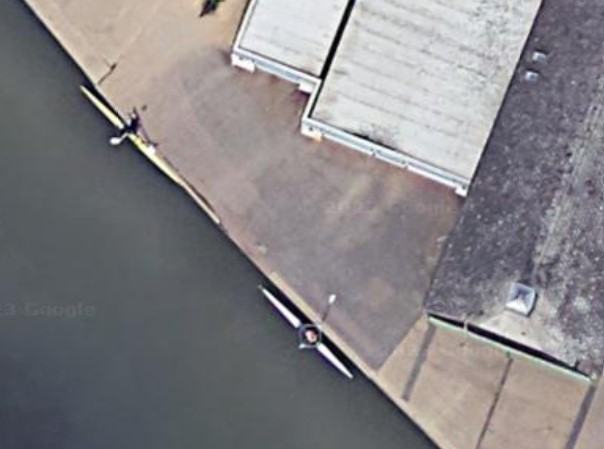
\includegraphics[scale=0.2]{earthSculler.jpg}
\end{center}
\end{figure}
\begin{figure}[h]
\caption{Rowing boats, potential obstacles and assumed connections marked on a Google Maps map of the river Thames}
\begin{center}
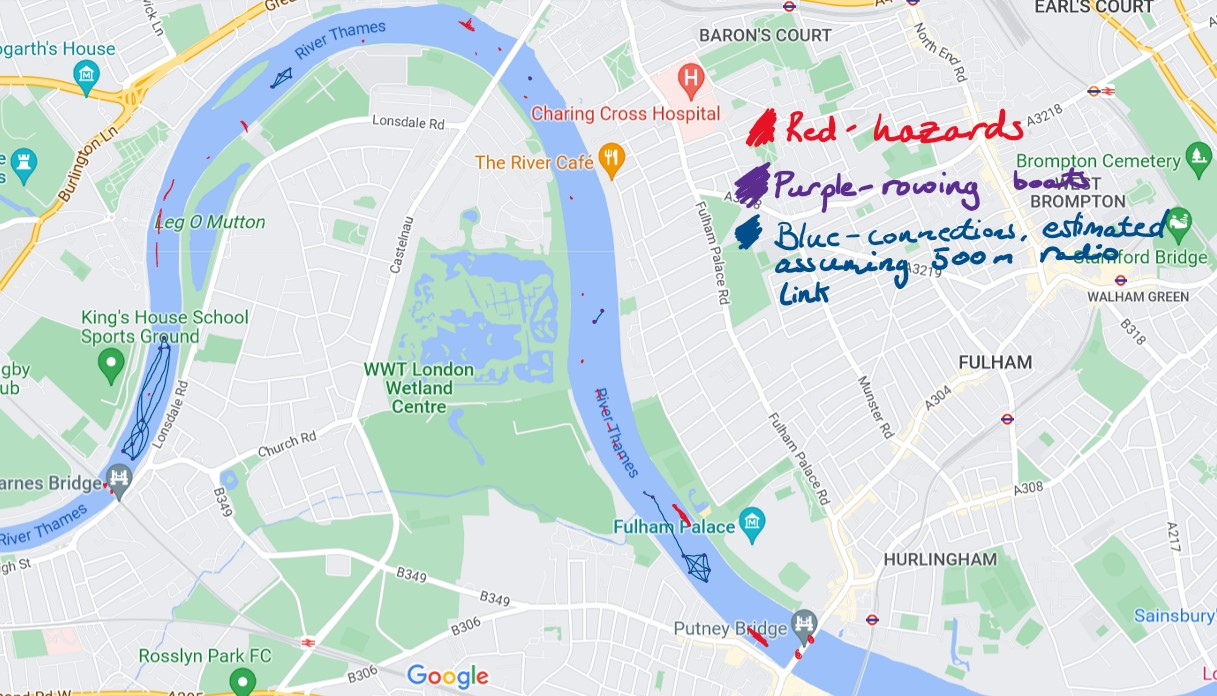
\includegraphics[scale=0.4]{mapsmarked.jpg}
\end{center}
\end{figure}
\begin{figure}[h]
\begin{center}
\caption{The network of rowing boats in an abstracted form}
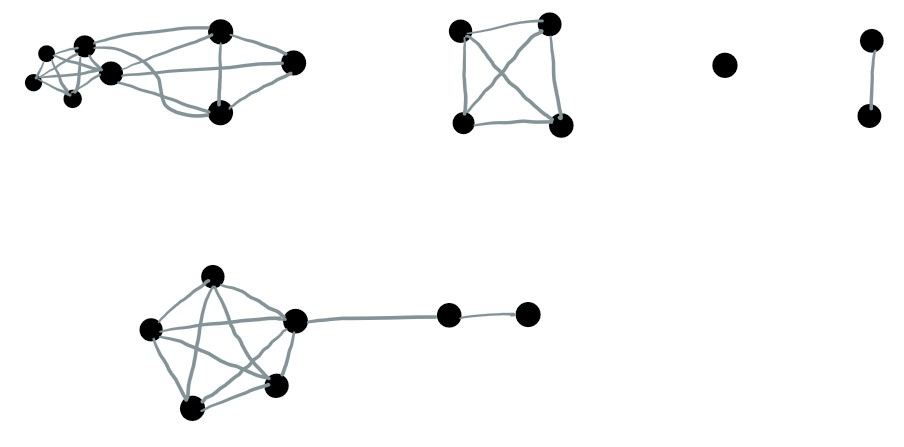
\includegraphics[scale=0.5]{lines.jpg}
\end{center}
\end{figure}
\FloatBarrier The final three requirements I identified as my success criteria were:
\begin{enumerate}
\item The Epidemic routing protocol is implemented on the network 
\item An application layer to demonstrate the utility of the network has been implemented
\item An evaluation of the performance of the network has been carried out
\end{enumerate}
All of these requirements have been implemented during this project. The finer details of this are in the Implementation chapter. \\ \\ I laid out several extension tasks. Some of them were drawn from my research into networking protocols other than Epidemic. For instance, I wanted to use a metric for transmission quality -- received strength signal indicator (RSSI) in radio communication -- to influence whether an anti-entropy session was initiated. Additionally, the GPS location could be used, either by only contacting nearby nodes to increase the probability that an anti-entropy session is successful, or prioritising sending messages about new obstacles to nodes that are near these obstacles. While time constraints have not allowed me to implement these extensions, I have implemented an extension allowing messages to have two priorities -- normal and urgent. This is also detailed in the Implementation chapter. 

\section{System Design}
Having decided on the Epidemic routing protocol, I planned the structure of the software that would run on each node. I knew that the Raspberry Pi Pico uses the RP2040 chip, containing two cores. To make best use of the hardware, I decided to design application and networking threads that would run on each core, with global data structures and concurrency control to pass messages between the two layers and allow both of them to access the GPS board. \\ \\
TODO you should talk about the flooding state machine you designed and the similarities between eidemic and flooding \\ \\ 
The application thread is responsible for notifying the user when they are too close to an obstacle. It also takes input from the user, generating new obstacles when a button is pressed. The initial state machine is shown in Figure 2.4. The a time to live (TTL) for each obstacle. If the object is permanent, such as a bridge, the TTL is set to $-1$, indicating that it should never be removed.
\begin{figure}[h]
\begin{center}
\caption{The initial state machine for the application thread}
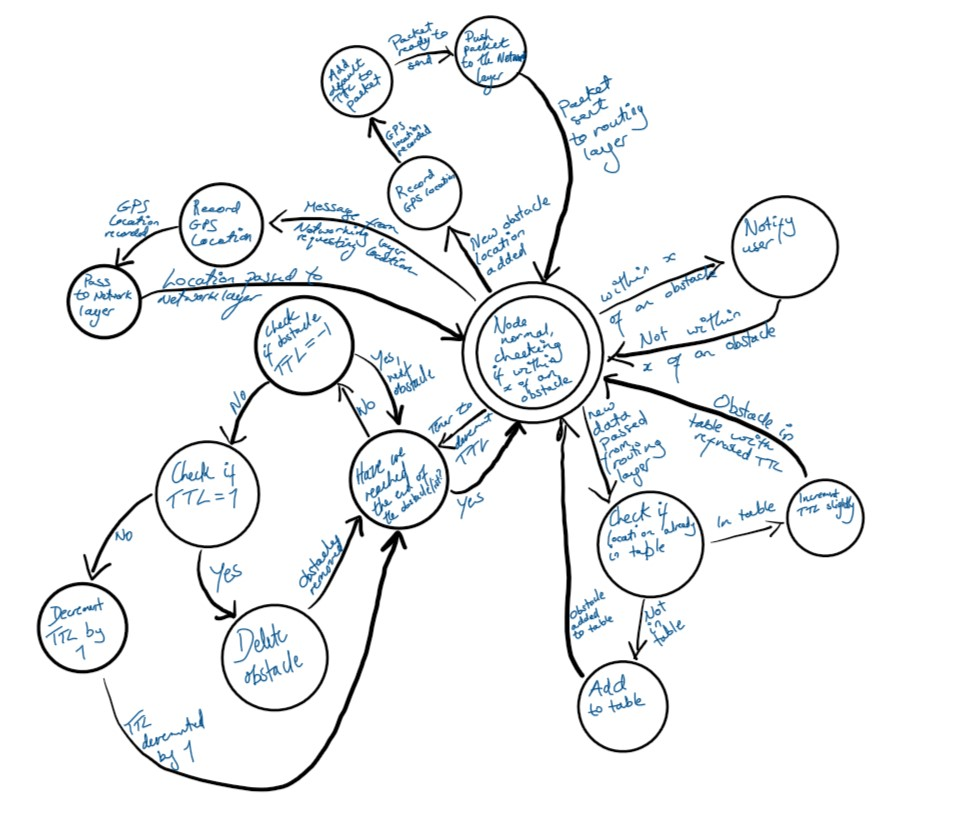
\includegraphics[scale=0.5]{appThread.jpg}
\end{center}
\end{figure}
\FloatBarrier
The networking thread contains the implementation of Epidemic with media access control. While routing and medium access control are typically handled separately -- in the OSI model they are in the second and third layers respectively -- they were considered together for my project to prevent work being repeated and use the limited computing resources available most effectively. This means that the implementation of Epidemic will also change. Not only will the node refuse to send any messages after hearing a CTS for a set period of time, or until it hears an ACK, I also integrated the message vector exchange at the start of an anti-entropy session into the CTS and RTS messages. This minimised the number of packets sent over the network, reducing the overall probability of collisions or errors in transmission. This state machine has changed slightly since it was first designed, with the changes and the decisions behind them being documented in the Implementation chapter. 
\begin{figure}[h]
\begin{center}
\caption{The initial state machine for the networking thread}
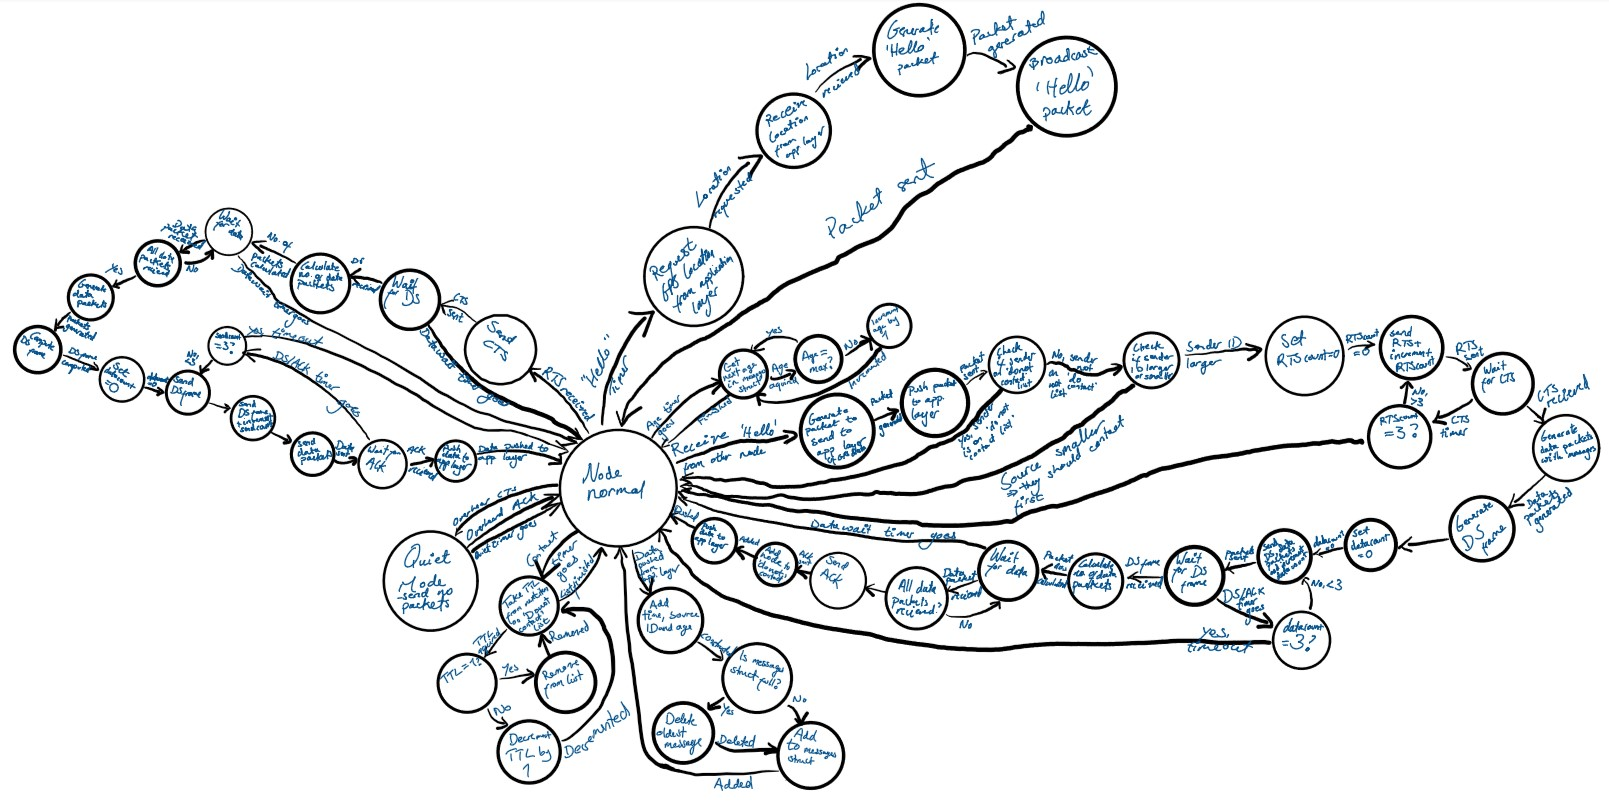
\includegraphics[scale=0.5]{net.jpg}
\end{center}
\end{figure}
\FloatBarrier
TODO -- talk about data structures -- The data structures designed to communicate messages between one thread and the other are  \\ \\
While these state machines were broadly implemented, the overall structure of the software changed, with only one thread running due to the limitations of CircuitPython and difficulties transitioning into MicroPython. This decision and the reasoning behind it is detailed in the Implementation chapter. 

%%% IMPLEMENTATION %%%
\newchapter{3}{Implementation}


%%% EVALUATION %%%
\newchapter{4}{Evaluation}
Evaluation was done (mostly) according to the plan in appendix. It was split into evaluation of the MANET and the whole system.

\section{Evaluating the MANET}
Break this down into smaller sections -- heavily quanitfy your results

\section{Evaluating the System}
We can def call this something better than the system? Idk the whole project, a more holistic evaluation? Emphasise that while the use case is kinda huge and untestable you tested within these restrictions and these parameters were met

%%% CONCLUSION %%%
\newchapter{5}{Conclusion}
What did this project do? The project met and exceeded the success criteria.

\section{Achievements}
What have you done?
In this project I have 

The evaluation shows that. This project is weak in. 

\section{Learning}
Aka lessons learnt / what I would do differently last time
Probably spent too much time researching BATMAN when it didn't really fit the parameters
Hardware is hard Just a stupid amount about radios and microprocessors

\section{Future Work}
I laid out several extension tasks. Some of them were drawn from my research into networking protocols other than Epidemic. For instance, I wanted to use a metric for transmission quality -- received strength signal indicator (RSSI) in radio communication -- to influence whether an anti-entropy session was initiated. Additionally, the GPS location could be used, either by only contacting nearby nodes to increase the probability that an anti-entropy session is successful, or prioritising sending messages about new obstacles to nodes that are near these obstacles. 
Encryption 
The success of my project will be defined by completion of the core criteria listed above. If there is
time, I have set further challenges:
1. Case studies on the path and timing of individual packets are performed
2. The network is further evaluated by examining the power consumption of individual nodes as
a proxy metric for traffic passing through a node
3. The User Interface of the device is evaluated
4. The application layer is further enhanced, using heuristics and extra data such as angle of
attack from GPS and combining sensor data
5. The routing layer is further enhanced by passing additional data, such as location awareness,
to the routing protocol
Okay so we never shut anything down in a safe ish way -- just kinda pull the plug and fuck off... ? Actually you should definately implement an editing of the Config file so we DO BETTER


%%% BIBLIOGRAPHY  %%%
\addcontentsline{toc}{chapter}{Bibliography}
%\bibliography{refs}


%%% APPENDICES %%%
\chapter*{Appendices}
\addcontentsline{toc}{chapter}{Appendices}  

\section*{A -- Guide to Building a Node}
\label{appendixA}
\addcontentsline{toc}{section}{A -- Guide to Building a Node}  
\setcounter{chapter}{0}
\setcounter{figure}{0}

\newpage
\section*{B -- Evaluation}
\label{appendixB}
\addcontentsline{toc}{section}{B -- Evaluation}  
\setcounter{figure}{0}
\documentclass[10pt, a4paper]{article}

% Template for a Computer Science Tripos Part II project dissertation
\documentclass[12pt,a4paper]{report}

% Gives a better chapter
\newcommand{\newchapter}[2]{
    \setcounter{chapter}{#1}
    \setcounter{section}{0}
    \chapter*{#2}
    \addcontentsline{toc}{chapter}{#1 #2}
}

\usepackage[pdfborder={0 0 0}]{hyperref}    % turns references into hyperlinks
\usepackage{verbatim}
\usepackage[utf8]{inputenc}
\usepackage{caption}
\usepackage{placeins}
\captionsetup{justification=raggedright,singlelinecheck=false}
\usepackage[none]{hyphenat}
\usepackage{graphicx}				% Allows for photos to be added
%\usepackage{parskip} 				% Stops the horrific spacing 
\usepackage[top=0cm, foot=1.5em, bottom=2.5cm, left=2cm, right=2cm]{geometry} 	% Set margins to .5 inches 
\addtolength{\topmargin}{0.5in}		% Set top margin to 1 inch
\usepackage{hyperref}				% Hyperlinks package
\hypersetup{colorlinks=true, linkcolor=blue, citecolor = blue, filecolor=black, urlcolor=blue} 	% Make types of hyperlinks
\urlstyle{same} 
\usepackage{pdfpages}				% Lets you add pdfs
\usepackage{caption}				% Captions
\usepackage[none]{hyphenat}			% Stops it splitting words over two lines 
\usepackage[OT1]{fontenc}		% Font
\renewcommand*\familydefault{\sfdefault} 
\usepackage{setspace}
\setstretch{1}
\usepackage{docmute}

%\graphicspath{}			if you have trouble getting images in the thing, asks for graphics in the same folder
%\usepackage{hhline}         			% Horizontal lines in tables
%\usepackage{siunitx}        			% Correct spacing of units
%\usepackage{amsmath}        			% American Mathematical Society
%\usepackage{amssymb}        			% Maths symbols
%\usepackage{amsthm}         			% Theorems
% \usepackage{lastpage}      			% ``n of m'' page numbering
%\usepackage{mathtools}
%\usepackage{changepage}
%\usepackage{blindtext}

%\raggedbottom                           % try to avoid widows and orphans
%\sloppy
%\clubpenalty1000%
%\widowpenalty1000%


\begin{document}
\bibliographystyle{plain}

%%% TITLE PAGE %%%
\thispagestyle{empty}

\rightline{\LARGE Alexandra Riddell-Webster}

\vspace*{60mm}
\begin{center}
\Huge
\textbf{A MANET to Facilitate Collision Avoidance in Rowing Boats} \\[5mm]
Computer Science Tripos -- Part II \\[5mm]
Murray Edwards College \\[5mm]
2023
\end{center}

%%% DECELERATION OF ORIGINALITY %%%
\pagestyle{plain}
\chapter*{Declaration of Originality}

I, Alexandra Riddell-Webster of Murray Edwards College, being a candidate for Part II of the Computer Science Tripos, hereby declare that this dissertation and the work described in it are my own work, unaided except as may be specified below, and that the dissertation does not contain material that has already been used to any substantial extent for a comparable purpose. \\ \\
I am content for my dissertation to be made available to the students and staff of the
University. \\

\bigskip
\leftline{\textbf{Signed:} Alexandra Riddell-Webster}
\leftline{\textbf{Date:} \today}

%%% ACKNOWLEDGEMENTS %%%
\chapter*{Acknowledgements}
This dissertation owes a huge amount to Matthew Ireland, for supervising me. My UTO, Jon Crowcroft was invaluable. Thanks to Cambridge University Boat Club, in particular Patrick Ryan, for allowing me to stick devices on rowing boats and for advising me on communication over water. I also thank Duncan Barnes for discussing GPS and electronics on rowing boats with me.



%%% PROFORMA %%%
\chapter*{Proforma}

{\large
\begin{tabular}{ll}
\bf Candidate Number:   & TODO \\
\bf Project Title:  & A MANET to Facilitate Collision Avoidance \\
& in Rowing Boats \\
\bf Examination:  & Computer Science Tripos -- Part II, May 2023      \\
\bf Word Count:    & TODO \footnotemark[1]   \\
\bf Code Line Count:    & TODO (inc. comments?) \\
\bf Project Originator: & Alexandra Riddell-Webster                 \\
\bf Supervisor:         & Mr Matthew Ireland  \\ 
\bf University Teaching Officer:  & Dr Jon Crowcroft \\ 
\end{tabular}
}
\footnotetext[1]{TODO} % This word count was computed by \texttt{detex diss.tex | tr -cd '0-9A-Za-z $\tt\backslash$n' | wc -w} }
\stepcounter{footnote}


\section*{Original Aims of the Project}
% At most 100 words on what this project aimed to do
TODO

\section*{Work Completed}
% 100 words on what I have done on this dis
TODO

\section*{Special Difficulties}
None.


%%% CONTENTS %%%
\newpage
{
\hypersetup{linkcolor=black}
\tableofcontents
}

%%% INTRODUCTION %%%
\newchapter{1}{Introduction}
This project built a mobile ad-hoc network (MANET) to facilitate collision avoidance amongst rowing boats. This MANET uses the geographic coordinates of boats and obstacles to determine if a boat is too close to an obstacle, then warns the user by buzzing or flashing an LED. A modified version of the Epidemic routing protocol has been implemented and nodes built to use it. The Evaluation chapter quantifies this implementation of Epidemic, then assesses the entire system. The Conclusion details further work that could be undertaken on the project. The project is open source, with a `how to' guide [\hyperref[appendixA]{Appendix A}] for construction of a node and the code available on the internet (TODO CITE) so any rowing club can use this as a collision avoidance tool.    

\section{Motivation}	
It is obvious that collisions between rowing boats and obstacles or other boats is unwanted, injuring rowers and causing equipment damage. While coxswains are responsible for steering a boat, they are fallible and may need extra assistance, particularly when steering in adverse conditions, such as fog. Coxless boats are at greater risk of collision, where rowers, facing away from the direction of travel, are responsible for steering boats. This project can be used in both coxed and coxless boats. \\
This project has a very personal motivation, as a friend was hit by an eight while in a single three years ago, causing a severe concussion that resulted in two years of intermission from her studies. \\ \\
This project produces devices designed to reduce the number and severity of collisions, warning users before they crash. While researching this project, I found a previous attempt to solve the problem, ROWCUS (TODO cite Rowcus). ROWCUS produced a device with radar to detect potential collisions. It seems to have proven commercially inviable, as the company states they ``have decided to not pursue the commercial deployment of ROWCUS'' (TODO cite). I am a proponent of open source, so the project is available entirely online. This includes a `how to' guide to building a node [\hyperref[appendixA]{Appendix A}], so others can build the solution.

\section{Related Work}
As mentioned above, ROWCUS (TODO cite) has attempted to solve this problem with a different technical solution -- using radar rather than GPS to detect proximity to obstacles, and without networking. While ROWCUS has similar goals to my project, the technical methodologies are different. The main differences are use of GPS and networking -- my project connects nodes together while ROWCUS has individual nodes. \\ \\
The nodes in my project communicate known obstacles to each other. Vahdat and Becker's paper `Epidemic Routing for Partially-Connected Ad Hoc Networks' is the key paper used to implement routing within the MANET. The term `anti-entropy' as used in my dissertation, comes from this paper. An anti-entropy session occurs when two nodes come into communication range and exchange messages. While the implementation in my project differs from this paper in some areas, including medium access control (detailed in the Preparation and Implementation chapters), this paper forms the foundation for the project. 



%%% PREPARATION %%%
\newchapter{2}{Preparation}
This chapter is laid out in chronological order. It first details the work done before the start of term, then the analysis that lead me to decide on the Epidemic routing protocol, particularly analysis of the structure of the networks rowing boats generate. This chapter finishes with the state machines designed after the project was accepted.

\section{Starting Point} 
Previous to this project, I had no hands-on experience with microcontrollers, although I had worked with Raspberry Pi single board computers. I had previously worked with AdaFruit components, however not with the radio and GPS boards used in this project. I therefore dedicated a small amount of time over the summer to learning about microprocessors and MicroPython, completing basic tasks such as flashing an onboard LED. In hindsight, while this was useful, my project is implemented in CircuitPython, so it would have been more beneficial to have explored this. \\ 
Before term started I felt it was important to verify the hardware I would use, particularly as there were chip shortages at the time. I therefore ordered and ran basic tests on the Raspberry Pi Picos and AdaFruit RFM69 radio and GPS boards. I chose to use AdaFruit and Raspberry Pi boards as there is a strong community surrounding the hardware, and the AdaFruit boards are supported by open source libraries that allow rudimentary operations to be performed. \\ \\ 
I had some experience with networking and routing protocols prior to starting this project. This was composed of the Part IB networking module and a small amount of work during an internship. Throughout the course of my project I took the Part II principles of communications course, further expanding my knowledge. I also researched MANETs and their corresponding networking protocols during the summer vacation. Most of this research was centred around the Better Approach to Ad-Hoc Mobile Networking (BATMAN) protocol (TODO cite) and other networking protocols that are not delay-tolerant. My project implemented an extended version of the Epidemic routing protocol from scratch. 


\section{Networking}
A MANET is characterised by wireless nodes, a frequently changing network topology and no reliance on pre-existing infrastructure. They are decentralised and therefore have no single point of failure (TODO cite D2). MANETs have a large range of uses, such as facilitating communication in military conflicts (TODO cite D3) to autonomous vehicles (TODO D4) and disaster relief scenarios where previously existing infrastructure is destroyed (TODO cite D5). This project constructs a MANET due to the lack of pre-existing infrastructure and the difficulties associated with setting up and maintaining a base station or similar. Requiring an infrastructure like this would also raise the barrier for entry for many clubs with limited funds and technical skills. \\ \\
Routing protocols find a path from a source to one or more destinations destination within the network. Different routing protocols optimise different parameters, and are better suited for different network topologies and applications (TODO cite princomm lecture notes). Within MANETs, a routing protocol must allow the network topology to change over time. They tend to contain node discovery techniques to allow for this. \\ \\
Before deciding on Epidemic as the routing protocol to implement for my project, I considered several other protocols. The the Better Approach to Ad-Hoc Mobile Networking (BATMAN) protocol (TODO cite) designed to route messages through MANETs, broadcasting originator messages (OGM) for node discovery. BATMAN has the interesting addition of a transmit quality (TQ) metric in the OGM packets, allowing the quality of connections between nodes to be factored into the route packets take through the network. While BATMAN does allow messages to be broadcast to all nodes, its primary focus is routing messages from one node to another. Additionally, while it allows for message mobility, it is not delay-tolerant.\\ \\
Another routing protocol examined was Greedy Perimeter Stateless Routing (GPSR), a location based routing protocol (TODO cite). GPSR exploits the relation between geographic position and connectivity in a wireless network, where each node tells its immediate neighbours its current location. Greedy forwarding is predominantly used to send packets to nodes that are progressively closer to the destination, until the destination coordinates can be reached. Where greedy forwarding fails, GPSR uses perimeter forwarding (forwarding the packets around the perimeter of the region) until greedy forwarding can be used again. This protocol was ultimately deemed to be unsuitable for my project as, similarly to BATMAN, its primary focus is in sending messages between two nodes. Additionally, the high mobility of the nodes in the use case means that forwarding packets to a set of coordinates does not mean the message will reach the intended destination, as the node may have moved. \\ \\ 
I chose to implement Epidemic in my project. Epidemic routing gains its names from its similarity to the spreading of infections. Each node replicates and transmits messages to neighbours that have not recently been contacted. These neighbours are discovered when each node broadcasts its existence to its neighbours. Epidemic was implemented in this project because it is a delay-tolerant routing protocol and best fits the likely network topology generated by rowing boats, as detailed in the Requirements section below. The networks generated by rowing boats have a high chance of partition, but the nodes are highly mobile. As Epidemic allows any node to carry network information it is best suited to the network.  Also something about how Epidemic does not route messages node to node but rather everywhere which is better suited to the use case. \\ \\
%TODO -- write a hell of a lot more about Epidemic. Write about an anti-entropy session properly
While these routing protocols often have mechanisms to minimise the probability of collisions, such as adding a jitter in the sending of discovery messages, none of them contain medium access control. Due to the probability of collisions between messages causing disruption to the sending of messages, particularly as all nodes are broadcasting on the same radio frequency (433 MHz). It was  therefore prudent to include media access control in the system. Multiple Access with Collision Avoidance for Wireless (MACAW) is often used by ad-hoc networks. MACAW uses request to send (RTS) and clear to send (CTS) messages to minimise the probability of collision. As discussed in the System Design section, MACAW inspired the medium access control in my project. 

\section{Project Development} 
This project was structured using the waterfall model for software development. The project proposal [\hyperref[appendixD]{Appendix D}] lays out the phases of the project and the output from each stage in a plan of work. The waterfall model of software development was used as it lends itself to the structure of a dissertation, with the five stages: \\
\centerline{Requirements $\rightarrow$ System Design $\rightarrow$ Implementation $\rightarrow$ Testing $\rightarrow$ Maintenance} \\ \\
This project used CircuitPython, as it is compatible with the existing AdaFruit libraries I used and extended in the project, and can easily be run on the Raspberry Pi Pico. \\ \\
GitHub was used to perform version control on the code and dissertation for this project. This also allowed me to fork repositories and submit a pull request to AdaFruit. \\ \\ 
TODO -- VS code and pylint so you don't have to run the code on the device to find out if it is correct 

\section{Requirements}
My requirements were based around the use case for the project -- as devices attached to rowing boats. This factored into my hardware decisions, as I wanted to use small and relatively lightweight items. Additionally, I chose to use the 433 MHz band as it is free to use without licencing, allowing me and other rowing clubs to use it without additional bureaucracy. \\ \\ 
The potential topology of the network was then analysed. This was done by looking at example distributions of rowing boats on lakes and rivers. One potential use case for this network that I am familiar with is the river Thames. Below I have analysed Google Maps and Earth's satellite view of the Thames along a 5.5km stretch of the Championship Course, pinpointing rowing boats and coaching launches, then adding them to a map with potential connections between nodes, assuming the radios have a range of 500m, alongside obstacles. This process is shown in Figures 2.1 and 2.2. I then abstracted this to the network topology of these rowing boats, shown in Figure 2.3.
\begin{figure}[h]
\caption{A rowing boat seen on Google Earth (TODO cite)}
\begin{center}
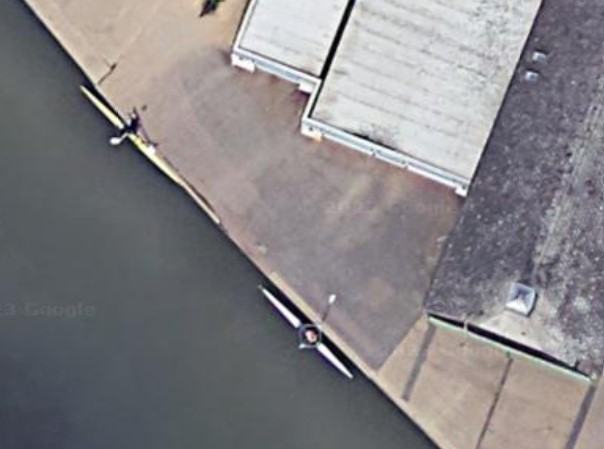
\includegraphics[scale=0.2]{earthSculler.jpg}
\end{center}
\end{figure}
\begin{figure}[h]
\caption{Rowing boats, potential obstacles and assumed connections marked on a Google Maps map of the river Thames}
\begin{center}
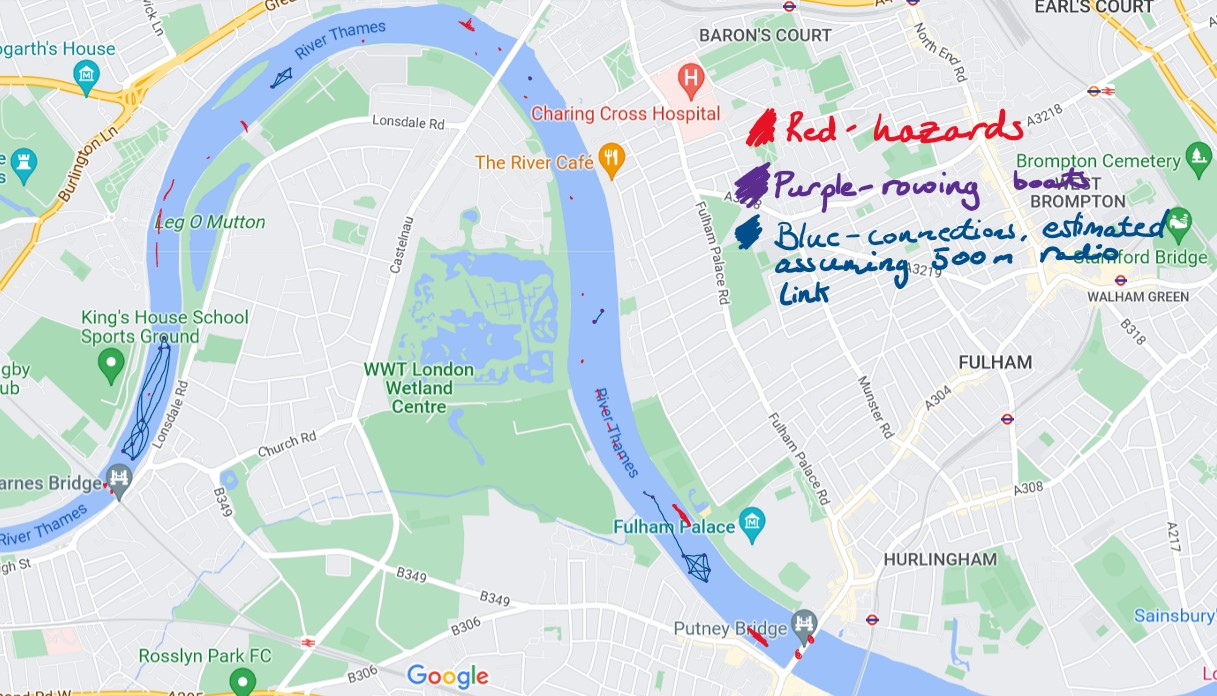
\includegraphics[scale=0.4]{mapsmarked.jpg}
\end{center}
\end{figure}
\begin{figure}[h]
\begin{center}
\caption{The network of rowing boats in an abstracted form}
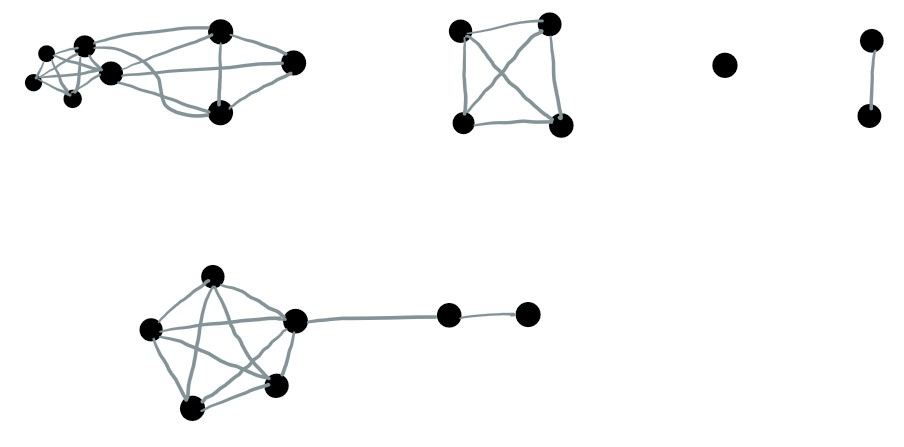
\includegraphics[scale=0.5]{lines.jpg}
\end{center}
\end{figure}
\FloatBarrier The final three requirements I identified as my success criteria were:
\begin{enumerate}
\item The Epidemic routing protocol is implemented on the network 
\item An application layer to demonstrate the utility of the network has been implemented
\item An evaluation of the performance of the network has been carried out
\end{enumerate}
All of these requirements have been implemented during this project. The finer details of this are in the Implementation chapter. \\ \\ I laid out several extension tasks. Some of them were drawn from my research into networking protocols other than Epidemic. For instance, I wanted to use a metric for transmission quality -- received strength signal indicator (RSSI) in radio communication -- to influence whether an anti-entropy session was initiated. Additionally, the GPS location could be used, either by only contacting nearby nodes to increase the probability that an anti-entropy session is successful, or prioritising sending messages about new obstacles to nodes that are near these obstacles. While time constraints have not allowed me to implement these extensions, I have implemented an extension allowing messages to have two priorities -- normal and urgent. This is also detailed in the Implementation chapter. 

\section{System Design}
Having decided on the Epidemic routing protocol, I planned the structure of the software that would run on each node. I knew that the Raspberry Pi Pico uses the RP2040 chip, containing two cores. To make best use of the hardware, I decided to design application and networking threads that would run on each core, with global data structures and concurrency control to pass messages between the two layers and allow both of them to access the GPS board. \\ \\
TODO you should talk about the flooding state machine you designed and the similarities between eidemic and flooding \\ \\ 
The application thread is responsible for notifying the user when they are too close to an obstacle. It also takes input from the user, generating new obstacles when a button is pressed. The initial state machine is shown in Figure 2.4. The a time to live (TTL) for each obstacle. If the object is permanent, such as a bridge, the TTL is set to $-1$, indicating that it should never be removed.
\begin{figure}[h]
\begin{center}
\caption{The initial state machine for the application thread}
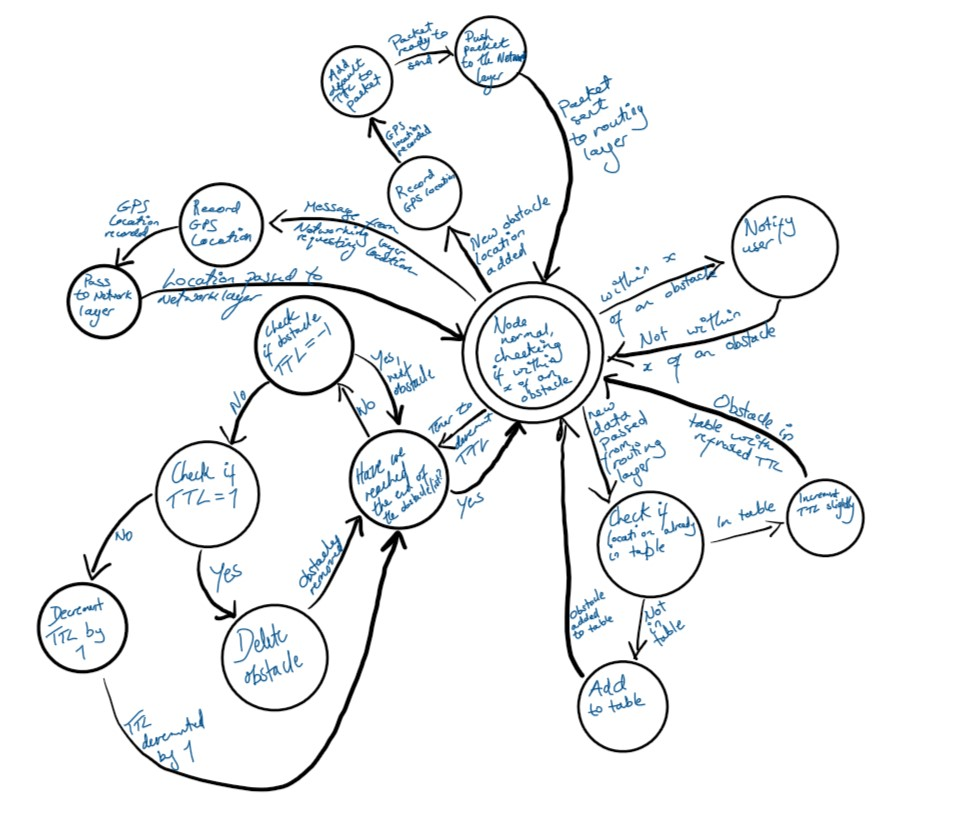
\includegraphics[scale=0.5]{appThread.jpg}
\end{center}
\end{figure}
\FloatBarrier
The networking thread contains the implementation of Epidemic with media access control. While routing and medium access control are typically handled separately -- in the OSI model they are in the second and third layers respectively -- they were considered together for my project to prevent work being repeated and use the limited computing resources available most effectively. This means that the implementation of Epidemic will also change. Not only will the node refuse to send any messages after hearing a CTS for a set period of time, or until it hears an ACK, I also integrated the message vector exchange at the start of an anti-entropy session into the CTS and RTS messages. This minimised the number of packets sent over the network, reducing the overall probability of collisions or errors in transmission. This state machine has changed slightly since it was first designed, with the changes and the decisions behind them being documented in the Implementation chapter. 
\begin{figure}[h]
\begin{center}
\caption{The initial state machine for the networking thread}
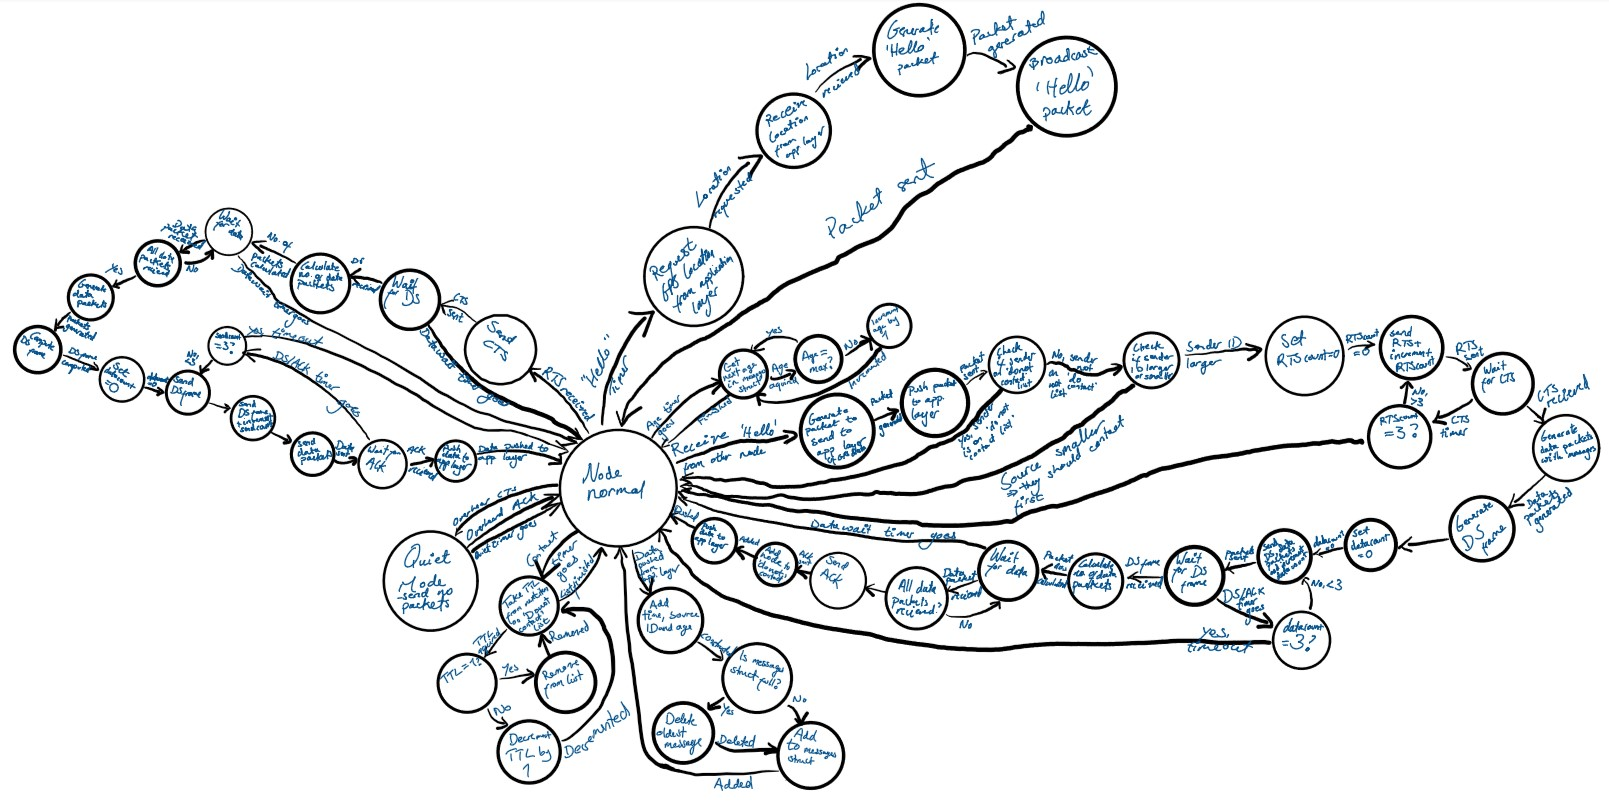
\includegraphics[scale=0.5]{net.jpg}
\end{center}
\end{figure}
\FloatBarrier
TODO -- talk about data structures -- The data structures designed to communicate messages between one thread and the other are  \\ \\
While these state machines were broadly implemented, the overall structure of the software changed, with only one thread running due to the limitations of CircuitPython and difficulties transitioning into MicroPython. This decision and the reasoning behind it is detailed in the Implementation chapter. 

%%% IMPLEMENTATION %%%
\newchapter{3}{Implementation}


%%% EVALUATION %%%
\newchapter{4}{Evaluation}
Evaluation was done (mostly) according to the plan in appendix. It was split into evaluation of the MANET and the whole system.

\section{Evaluating the MANET}
Break this down into smaller sections -- heavily quanitfy your results

\section{Evaluating the System}
We can def call this something better than the system? Idk the whole project, a more holistic evaluation? Emphasise that while the use case is kinda huge and untestable you tested within these restrictions and these parameters were met

%%% CONCLUSION %%%
\newchapter{5}{Conclusion}
What did this project do? The project met and exceeded the success criteria.

\section{Achievements}
What have you done?
In this project I have 

The evaluation shows that. This project is weak in. 

\section{Learning}
Aka lessons learnt / what I would do differently last time
Probably spent too much time researching BATMAN when it didn't really fit the parameters
Hardware is hard Just a stupid amount about radios and microprocessors

\section{Future Work}
I laid out several extension tasks. Some of them were drawn from my research into networking protocols other than Epidemic. For instance, I wanted to use a metric for transmission quality -- received strength signal indicator (RSSI) in radio communication -- to influence whether an anti-entropy session was initiated. Additionally, the GPS location could be used, either by only contacting nearby nodes to increase the probability that an anti-entropy session is successful, or prioritising sending messages about new obstacles to nodes that are near these obstacles. 
Encryption 
The success of my project will be defined by completion of the core criteria listed above. If there is
time, I have set further challenges:
1. Case studies on the path and timing of individual packets are performed
2. The network is further evaluated by examining the power consumption of individual nodes as
a proxy metric for traffic passing through a node
3. The User Interface of the device is evaluated
4. The application layer is further enhanced, using heuristics and extra data such as angle of
attack from GPS and combining sensor data
5. The routing layer is further enhanced by passing additional data, such as location awareness,
to the routing protocol
Okay so we never shut anything down in a safe ish way -- just kinda pull the plug and fuck off... ? Actually you should definately implement an editing of the Config file so we DO BETTER


%%% BIBLIOGRAPHY  %%%
\addcontentsline{toc}{chapter}{Bibliography}
%\bibliography{refs}


%%% APPENDICES %%%
\chapter*{Appendices}
\addcontentsline{toc}{chapter}{Appendices}  

\section*{A -- Guide to Building a Node}
\label{appendixA}
\addcontentsline{toc}{section}{A -- Guide to Building a Node}  
\setcounter{chapter}{0}
\setcounter{figure}{0}

\newpage
\section*{B -- Evaluation}
\label{appendixB}
\addcontentsline{toc}{section}{B -- Evaluation}  
\setcounter{figure}{0}
\input{evaluationPlan}

\newpage
\section*{C -- Progress Report}
\label{appendixC}
\addcontentsline{toc}{section}{C -- Progress Report}  
\setcounter{figure}{0}
\input{progressReport}

\newpage
\section*{D -- Project Proposal}
\label{appendixD}
\addcontentsline{toc}{section}{D -- Project Proposal}  
\setcounter{figure}{0}
\input{phase3}

\end{document}
%\frenchspacing			to get rid of the double spaces after full stops
%\graphicspath{}			if you have trouble getting images in the thing, asks for graphics in the same folder
\usepackage{caption}
\usepackage{placeins}
\captionsetup{justification=raggedright,singlelinecheck=false}
\usepackage[none]{hyphenat}

\begin{document}
\begin{center}
\Huge{Part II Project - Plan for Evaluation} \par
\Large{\today} \par
\end{center}
\par
\par

\section{Overview}
The evaluation for the mobile ad-hoc network (MANET) will be split into two parts -- first the evaluation for the pure MANET and a whole system evaluation. The evaluation of the MANET will examine the implementation of Epidemic, the delay tolerant networking protocol will be checked for correctness and performance. The system evaluation will look at the MANET in the context of the use case, on the water.  \\

All data will be logged on the node in a CSV file with columns \\ \verb'Node Address, Time, Time Since Node Startup, Event Type, Event Information' \\ where the Event Information varies with the event being logged and may contain the GPS location and message keys. This data will then be analysed on my device using Python code.

\section{Evaluating the MANET}
These tests be conducted in a field, as this will give an outdoor environment similar to the use case, but I will be able to better control the conditions the node is in. They will use four nodes, as this is the maximum number of nodes we can accurately calculate time for. Two nodes will use GPS to find the current time and two will use the serial connection to laptops to calculate the time. These tests will be conducted first on a small scale, with short tests using a small number of nodes, to ensure the tests can be run. After this has been confirmed, the tests will be run for a longer time with the maximum number of nodes. 

The tests can then be compared to the evaluation in the initial epidemic paper \cite{epidemic}, which simulated the nodes with 50 mobile nodes in a 1500 x 300 m space using the Monarch extensions to the ns-2 packet-level simulator rather than hardware as I am doing. Evaluation metrics examined included message delivery latency, delivery rate, the average and maximum number of hops a message took to get to a node.

The first test will be the percentage of packets delivered in the four node network. This will be time limited (i.e. if a message is not received in x minutes, it is considered undelivered). Nodes will randomly generate a new message every second, for a total of 25 messages, mirroring the structure of testing used in Vahdat and Becker's paper \cite{epidemic}. The nodes will be in a box of area $20m^2$ with the range of the radios reduced to approximately $5m$ to simulate the environment in which the system will be used. The nodes will move constantly.

Next, the transfer delay will be measured. This will be the average time taken for each message to be delivered, and will use the same setup as percentage of packets delivered testing.

\begin{figure}[h]
\caption{The setup and axes for delivery rate and transfer delay}
\begin{center}
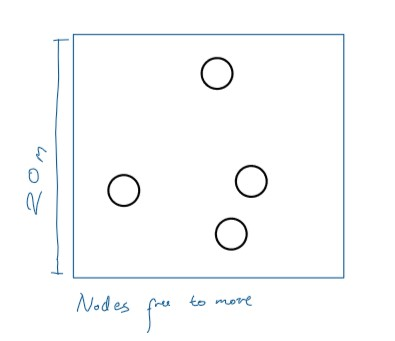
\includegraphics[scale=0.5]{transfer.jpg}
\end{center}
\end{figure}


Finally, the time taken to propagate messages after partition will be measured. This will include one-sided, asymmetric partitions, where only one set of nodes has messages the other set has not seen. It will also include symmetric partitions, where both sets of nodes have messages the other set has not seen. The number of unseen messages will be increased and each test will be run five times.

\begin{figure}[h]
\caption{The setup and axes for partition testing}
\begin{center}
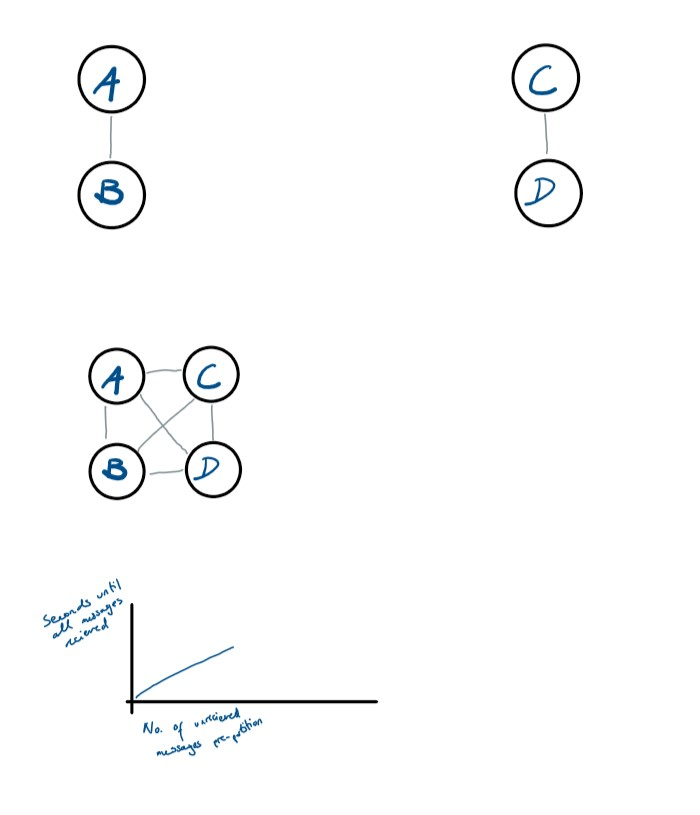
\includegraphics[scale=0.3]{partition.jpg}
\end{center}
\end{figure}


%sketch out graphs you will use
%Add pictures of the node teting setup 
%What will be evaluated and how?
%How to evaluate correctness? 
%How to do sensitivity on the data / metrics - how certain are we that this works..? 

\FloatBarrier
\section{Evaluating the System}
This will be performed on the water, the environment the MANET will be used in, after a `dry run' on land to ensure there are no obvious flaws with the system. 
To examine the use of the system and how long it takes messages to arrive at other nodes, a well known obstacle has been selected. This is the red buoy at 51.48236626931181, -0.22641424521527762, shown below \cite{maps}. Using the time given from the GPS chips, we can then map the locations and time since the obstacle was added that other nodes receive messages about the buoy. This experiment will be run multiple times to gather a sufficient volume of data about the propagation of new obstacles. \\

Additionally, this will allow me to look at the behaviour of users when adding a new obstacle then tweak the MANET to fit. While there is a ground truth about the location of an obstacle, it is likely that most users will not be directly above the obstacle when they log it. 

\begin{figure}[h]
\caption{The location of the `red buoy' obstacle \cite{maps}}
\begin{center}
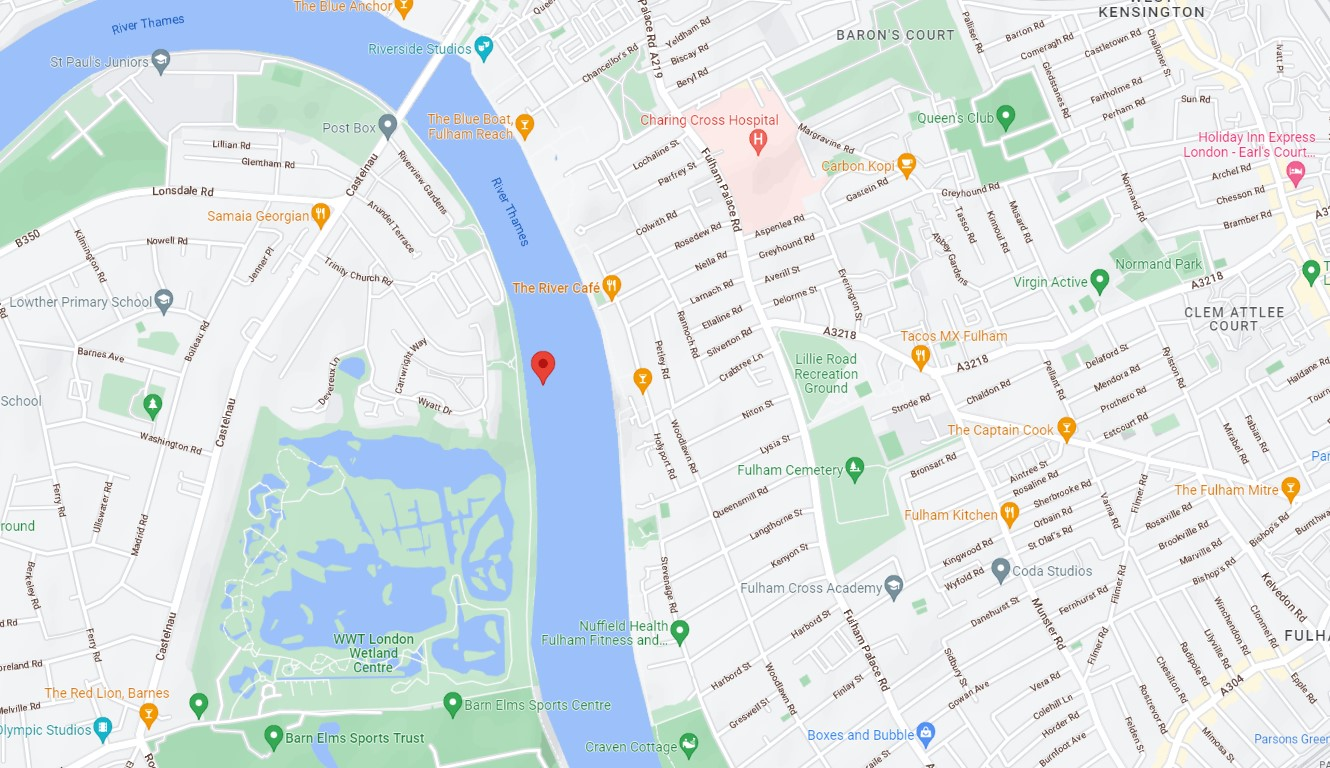
\includegraphics[scale=0.3]{buoy.jpg}
\end{center}
\end{figure}

\begin{figure}[h]
\caption{An image of the `red buoy' obstacle \cite{myphoto}}
\begin{center}
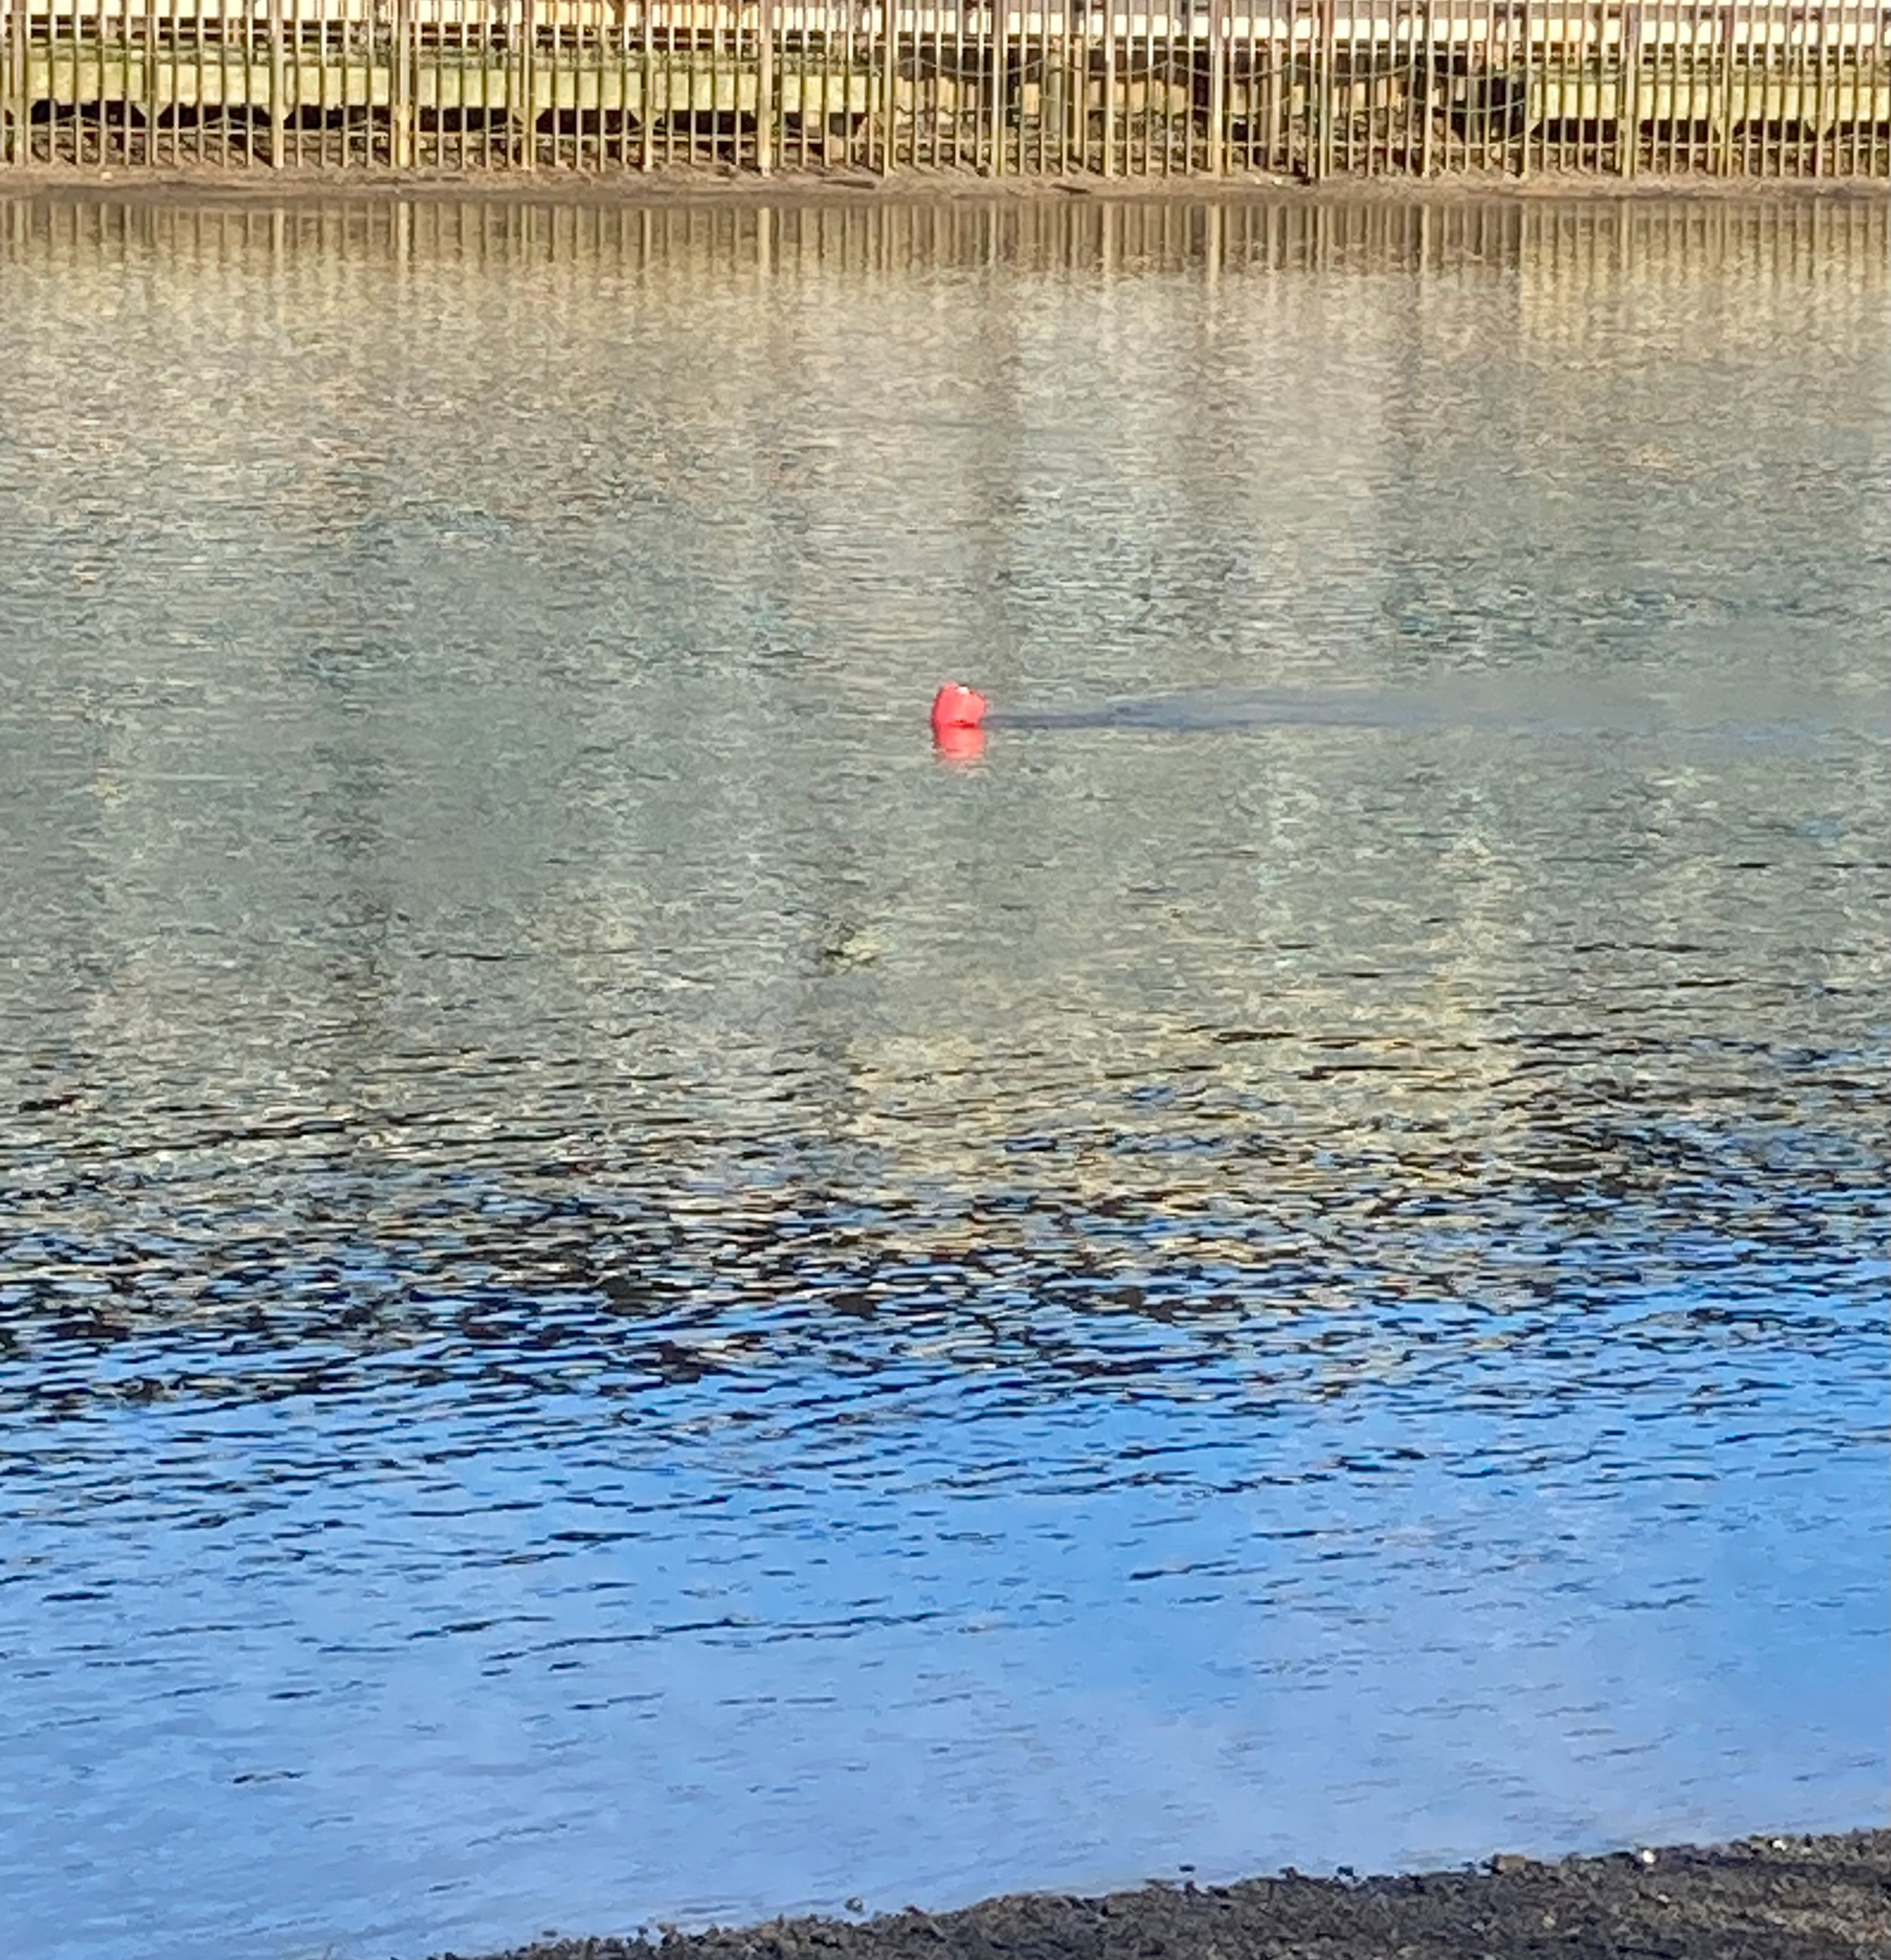
\includegraphics[scale=0.1]{buoy2.jpg}
\end{center}
\end{figure}
\FloatBarrier


\section{Extensions}
If there is sufficient time, further evaluation can be performed on the MANET. This will be structured in a similar way to the tests in the `Evaluating the MANET'. Bandwidth will be tested in a fully connected network, where the number of messages per second transferred between two nodes may be found by generating random packets at set intervals at one node (node A shown below), and seeing how many are passed to another node (node B below). 
This test could then be performed with both nodes generating and receiving messages, to examine bandwidth on a two way connection.\\
\begin{figure}[h]
\caption{The setup and expected graph for testing bandwidth}
\begin{center}
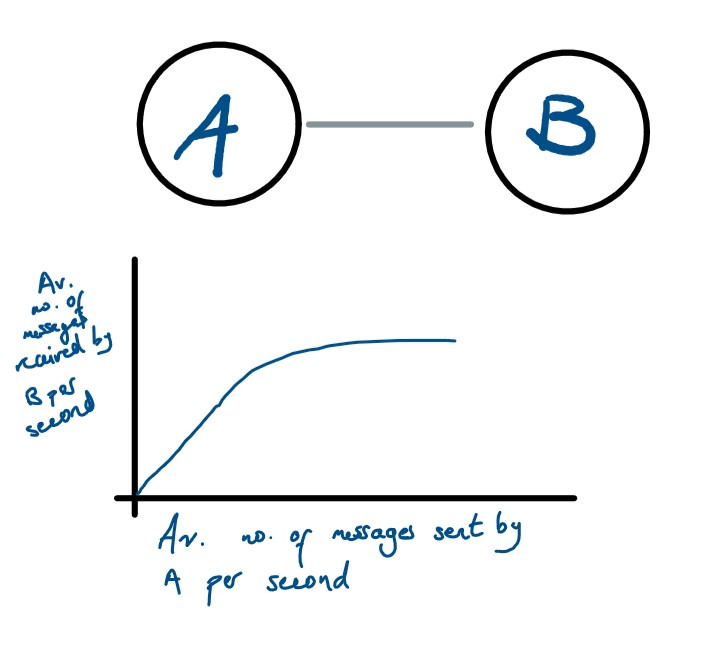
\includegraphics[scale=0.3]{bandwidth.jpg}
\end{center}
\end{figure}

Further extensions to the system evaluation will include a questionnaire for those who use the device, covering a range of users, including both coxes in coxed boats and rowers in coxless boats. 

\FloatBarrier
\vspace{10px}
\begin{thebibliography}{9} 
\bibitem{maps}Google Maps. 51.4823, -0.2264. [Online] Available at: \url{https://www.google.co.uk/maps/place/51%C2%B028'56.5%22N+0%C2%B013'35.1%22W/@51.4820341,-0.2295313,15.5z/data=!4m4!3m3!8m2!3d51.4823663!4d-0.2264142!5m1!1e4} [Accessed March 2023]

\bibitem{myphoto}Riddell-Webster, A. Red buoy. Taken March 2023. 

\bibitem{epidemic} Vahdat, A, Becker, D. Epidemic Routing for Partially-Connected Ad Hoc Networks. Published 2000. Duke University.
\end{thebibliography}

\end{document}








\newpage
\section*{C -- Progress Report}
\label{appendixC}
\addcontentsline{toc}{section}{C -- Progress Report}  
\setcounter{figure}{0}
\documentclass[10pt, a4paper]{article}

% Template for a Computer Science Tripos Part II project dissertation
\documentclass[12pt,a4paper]{report}

% Gives a better chapter
\newcommand{\newchapter}[2]{
    \setcounter{chapter}{#1}
    \setcounter{section}{0}
    \chapter*{#2}
    \addcontentsline{toc}{chapter}{#1 #2}
}

\usepackage[pdfborder={0 0 0}]{hyperref}    % turns references into hyperlinks
\usepackage{verbatim}
\usepackage[utf8]{inputenc}
\usepackage{caption}
\usepackage{placeins}
\captionsetup{justification=raggedright,singlelinecheck=false}
\usepackage[none]{hyphenat}
\usepackage{graphicx}				% Allows for photos to be added
%\usepackage{parskip} 				% Stops the horrific spacing 
\usepackage[top=0cm, foot=1.5em, bottom=2.5cm, left=2cm, right=2cm]{geometry} 	% Set margins to .5 inches 
\addtolength{\topmargin}{0.5in}		% Set top margin to 1 inch
\usepackage{hyperref}				% Hyperlinks package
\hypersetup{colorlinks=true, linkcolor=blue, citecolor = blue, filecolor=black, urlcolor=blue} 	% Make types of hyperlinks
\urlstyle{same} 
\usepackage{pdfpages}				% Lets you add pdfs
\usepackage{caption}				% Captions
\usepackage[none]{hyphenat}			% Stops it splitting words over two lines 
\usepackage[OT1]{fontenc}		% Font
\renewcommand*\familydefault{\sfdefault} 
\usepackage{setspace}
\setstretch{1}
\usepackage{docmute}

%\graphicspath{}			if you have trouble getting images in the thing, asks for graphics in the same folder
%\usepackage{hhline}         			% Horizontal lines in tables
%\usepackage{siunitx}        			% Correct spacing of units
%\usepackage{amsmath}        			% American Mathematical Society
%\usepackage{amssymb}        			% Maths symbols
%\usepackage{amsthm}         			% Theorems
% \usepackage{lastpage}      			% ``n of m'' page numbering
%\usepackage{mathtools}
%\usepackage{changepage}
%\usepackage{blindtext}

%\raggedbottom                           % try to avoid widows and orphans
%\sloppy
%\clubpenalty1000%
%\widowpenalty1000%


\begin{document}
\bibliographystyle{plain}

%%% TITLE PAGE %%%
\thispagestyle{empty}

\rightline{\LARGE Alexandra Riddell-Webster}

\vspace*{60mm}
\begin{center}
\Huge
\textbf{A MANET to Facilitate Collision Avoidance in Rowing Boats} \\[5mm]
Computer Science Tripos -- Part II \\[5mm]
Murray Edwards College \\[5mm]
2023
\end{center}

%%% DECELERATION OF ORIGINALITY %%%
\pagestyle{plain}
\chapter*{Declaration of Originality}

I, Alexandra Riddell-Webster of Murray Edwards College, being a candidate for Part II of the Computer Science Tripos, hereby declare that this dissertation and the work described in it are my own work, unaided except as may be specified below, and that the dissertation does not contain material that has already been used to any substantial extent for a comparable purpose. \\ \\
I am content for my dissertation to be made available to the students and staff of the
University. \\

\bigskip
\leftline{\textbf{Signed:} Alexandra Riddell-Webster}
\leftline{\textbf{Date:} \today}

%%% ACKNOWLEDGEMENTS %%%
\chapter*{Acknowledgements}
This dissertation owes a huge amount to Matthew Ireland, for supervising me. My UTO, Jon Crowcroft was invaluable. Thanks to Cambridge University Boat Club, in particular Patrick Ryan, for allowing me to stick devices on rowing boats and for advising me on communication over water. I also thank Duncan Barnes for discussing GPS and electronics on rowing boats with me.



%%% PROFORMA %%%
\chapter*{Proforma}

{\large
\begin{tabular}{ll}
\bf Candidate Number:   & TODO \\
\bf Project Title:  & A MANET to Facilitate Collision Avoidance \\
& in Rowing Boats \\
\bf Examination:  & Computer Science Tripos -- Part II, May 2023      \\
\bf Word Count:    & TODO \footnotemark[1]   \\
\bf Code Line Count:    & TODO (inc. comments?) \\
\bf Project Originator: & Alexandra Riddell-Webster                 \\
\bf Supervisor:         & Mr Matthew Ireland  \\ 
\bf University Teaching Officer:  & Dr Jon Crowcroft \\ 
\end{tabular}
}
\footnotetext[1]{TODO} % This word count was computed by \texttt{detex diss.tex | tr -cd '0-9A-Za-z $\tt\backslash$n' | wc -w} }
\stepcounter{footnote}


\section*{Original Aims of the Project}
% At most 100 words on what this project aimed to do
TODO

\section*{Work Completed}
% 100 words on what I have done on this dis
TODO

\section*{Special Difficulties}
None.


%%% CONTENTS %%%
\newpage
{
\hypersetup{linkcolor=black}
\tableofcontents
}

%%% INTRODUCTION %%%
\newchapter{1}{Introduction}
This project built a mobile ad-hoc network (MANET) to facilitate collision avoidance amongst rowing boats. This MANET uses the geographic coordinates of boats and obstacles to determine if a boat is too close to an obstacle, then warns the user by buzzing or flashing an LED. A modified version of the Epidemic routing protocol has been implemented and nodes built to use it. The Evaluation chapter quantifies this implementation of Epidemic, then assesses the entire system. The Conclusion details further work that could be undertaken on the project. The project is open source, with a `how to' guide [\hyperref[appendixA]{Appendix A}] for construction of a node and the code available on the internet (TODO CITE) so any rowing club can use this as a collision avoidance tool.    

\section{Motivation}	
It is obvious that collisions between rowing boats and obstacles or other boats is unwanted, injuring rowers and causing equipment damage. While coxswains are responsible for steering a boat, they are fallible and may need extra assistance, particularly when steering in adverse conditions, such as fog. Coxless boats are at greater risk of collision, where rowers, facing away from the direction of travel, are responsible for steering boats. This project can be used in both coxed and coxless boats. \\
This project has a very personal motivation, as a friend was hit by an eight while in a single three years ago, causing a severe concussion that resulted in two years of intermission from her studies. \\ \\
This project produces devices designed to reduce the number and severity of collisions, warning users before they crash. While researching this project, I found a previous attempt to solve the problem, ROWCUS (TODO cite Rowcus). ROWCUS produced a device with radar to detect potential collisions. It seems to have proven commercially inviable, as the company states they ``have decided to not pursue the commercial deployment of ROWCUS'' (TODO cite). I am a proponent of open source, so the project is available entirely online. This includes a `how to' guide to building a node [\hyperref[appendixA]{Appendix A}], so others can build the solution.

\section{Related Work}
As mentioned above, ROWCUS (TODO cite) has attempted to solve this problem with a different technical solution -- using radar rather than GPS to detect proximity to obstacles, and without networking. While ROWCUS has similar goals to my project, the technical methodologies are different. The main differences are use of GPS and networking -- my project connects nodes together while ROWCUS has individual nodes. \\ \\
The nodes in my project communicate known obstacles to each other. Vahdat and Becker's paper `Epidemic Routing for Partially-Connected Ad Hoc Networks' is the key paper used to implement routing within the MANET. The term `anti-entropy' as used in my dissertation, comes from this paper. An anti-entropy session occurs when two nodes come into communication range and exchange messages. While the implementation in my project differs from this paper in some areas, including medium access control (detailed in the Preparation and Implementation chapters), this paper forms the foundation for the project. 



%%% PREPARATION %%%
\newchapter{2}{Preparation}
This chapter is laid out in chronological order. It first details the work done before the start of term, then the analysis that lead me to decide on the Epidemic routing protocol, particularly analysis of the structure of the networks rowing boats generate. This chapter finishes with the state machines designed after the project was accepted.

\section{Starting Point} 
Previous to this project, I had no hands-on experience with microcontrollers, although I had worked with Raspberry Pi single board computers. I had previously worked with AdaFruit components, however not with the radio and GPS boards used in this project. I therefore dedicated a small amount of time over the summer to learning about microprocessors and MicroPython, completing basic tasks such as flashing an onboard LED. In hindsight, while this was useful, my project is implemented in CircuitPython, so it would have been more beneficial to have explored this. \\ 
Before term started I felt it was important to verify the hardware I would use, particularly as there were chip shortages at the time. I therefore ordered and ran basic tests on the Raspberry Pi Picos and AdaFruit RFM69 radio and GPS boards. I chose to use AdaFruit and Raspberry Pi boards as there is a strong community surrounding the hardware, and the AdaFruit boards are supported by open source libraries that allow rudimentary operations to be performed. \\ \\ 
I had some experience with networking and routing protocols prior to starting this project. This was composed of the Part IB networking module and a small amount of work during an internship. Throughout the course of my project I took the Part II principles of communications course, further expanding my knowledge. I also researched MANETs and their corresponding networking protocols during the summer vacation. Most of this research was centred around the Better Approach to Ad-Hoc Mobile Networking (BATMAN) protocol (TODO cite) and other networking protocols that are not delay-tolerant. My project implemented an extended version of the Epidemic routing protocol from scratch. 


\section{Networking}
A MANET is characterised by wireless nodes, a frequently changing network topology and no reliance on pre-existing infrastructure. They are decentralised and therefore have no single point of failure (TODO cite D2). MANETs have a large range of uses, such as facilitating communication in military conflicts (TODO cite D3) to autonomous vehicles (TODO D4) and disaster relief scenarios where previously existing infrastructure is destroyed (TODO cite D5). This project constructs a MANET due to the lack of pre-existing infrastructure and the difficulties associated with setting up and maintaining a base station or similar. Requiring an infrastructure like this would also raise the barrier for entry for many clubs with limited funds and technical skills. \\ \\
Routing protocols find a path from a source to one or more destinations destination within the network. Different routing protocols optimise different parameters, and are better suited for different network topologies and applications (TODO cite princomm lecture notes). Within MANETs, a routing protocol must allow the network topology to change over time. They tend to contain node discovery techniques to allow for this. \\ \\
Before deciding on Epidemic as the routing protocol to implement for my project, I considered several other protocols. The the Better Approach to Ad-Hoc Mobile Networking (BATMAN) protocol (TODO cite) designed to route messages through MANETs, broadcasting originator messages (OGM) for node discovery. BATMAN has the interesting addition of a transmit quality (TQ) metric in the OGM packets, allowing the quality of connections between nodes to be factored into the route packets take through the network. While BATMAN does allow messages to be broadcast to all nodes, its primary focus is routing messages from one node to another. Additionally, while it allows for message mobility, it is not delay-tolerant.\\ \\
Another routing protocol examined was Greedy Perimeter Stateless Routing (GPSR), a location based routing protocol (TODO cite). GPSR exploits the relation between geographic position and connectivity in a wireless network, where each node tells its immediate neighbours its current location. Greedy forwarding is predominantly used to send packets to nodes that are progressively closer to the destination, until the destination coordinates can be reached. Where greedy forwarding fails, GPSR uses perimeter forwarding (forwarding the packets around the perimeter of the region) until greedy forwarding can be used again. This protocol was ultimately deemed to be unsuitable for my project as, similarly to BATMAN, its primary focus is in sending messages between two nodes. Additionally, the high mobility of the nodes in the use case means that forwarding packets to a set of coordinates does not mean the message will reach the intended destination, as the node may have moved. \\ \\ 
I chose to implement Epidemic in my project. Epidemic routing gains its names from its similarity to the spreading of infections. Each node replicates and transmits messages to neighbours that have not recently been contacted. These neighbours are discovered when each node broadcasts its existence to its neighbours. Epidemic was implemented in this project because it is a delay-tolerant routing protocol and best fits the likely network topology generated by rowing boats, as detailed in the Requirements section below. The networks generated by rowing boats have a high chance of partition, but the nodes are highly mobile. As Epidemic allows any node to carry network information it is best suited to the network.  Also something about how Epidemic does not route messages node to node but rather everywhere which is better suited to the use case. \\ \\
%TODO -- write a hell of a lot more about Epidemic. Write about an anti-entropy session properly
While these routing protocols often have mechanisms to minimise the probability of collisions, such as adding a jitter in the sending of discovery messages, none of them contain medium access control. Due to the probability of collisions between messages causing disruption to the sending of messages, particularly as all nodes are broadcasting on the same radio frequency (433 MHz). It was  therefore prudent to include media access control in the system. Multiple Access with Collision Avoidance for Wireless (MACAW) is often used by ad-hoc networks. MACAW uses request to send (RTS) and clear to send (CTS) messages to minimise the probability of collision. As discussed in the System Design section, MACAW inspired the medium access control in my project. 

\section{Project Development} 
This project was structured using the waterfall model for software development. The project proposal [\hyperref[appendixD]{Appendix D}] lays out the phases of the project and the output from each stage in a plan of work. The waterfall model of software development was used as it lends itself to the structure of a dissertation, with the five stages: \\
\centerline{Requirements $\rightarrow$ System Design $\rightarrow$ Implementation $\rightarrow$ Testing $\rightarrow$ Maintenance} \\ \\
This project used CircuitPython, as it is compatible with the existing AdaFruit libraries I used and extended in the project, and can easily be run on the Raspberry Pi Pico. \\ \\
GitHub was used to perform version control on the code and dissertation for this project. This also allowed me to fork repositories and submit a pull request to AdaFruit. \\ \\ 
TODO -- VS code and pylint so you don't have to run the code on the device to find out if it is correct 

\section{Requirements}
My requirements were based around the use case for the project -- as devices attached to rowing boats. This factored into my hardware decisions, as I wanted to use small and relatively lightweight items. Additionally, I chose to use the 433 MHz band as it is free to use without licencing, allowing me and other rowing clubs to use it without additional bureaucracy. \\ \\ 
The potential topology of the network was then analysed. This was done by looking at example distributions of rowing boats on lakes and rivers. One potential use case for this network that I am familiar with is the river Thames. Below I have analysed Google Maps and Earth's satellite view of the Thames along a 5.5km stretch of the Championship Course, pinpointing rowing boats and coaching launches, then adding them to a map with potential connections between nodes, assuming the radios have a range of 500m, alongside obstacles. This process is shown in Figures 2.1 and 2.2. I then abstracted this to the network topology of these rowing boats, shown in Figure 2.3.
\begin{figure}[h]
\caption{A rowing boat seen on Google Earth (TODO cite)}
\begin{center}
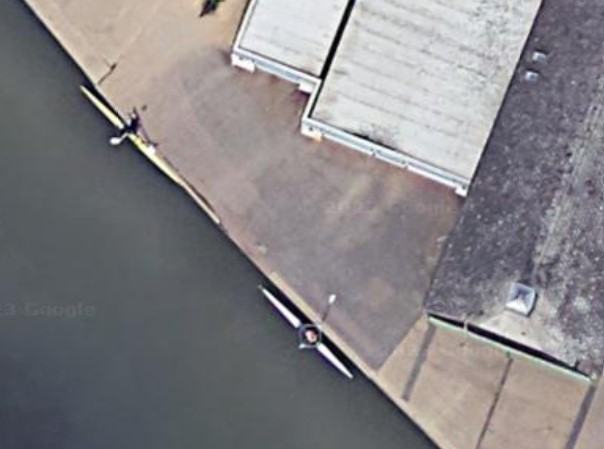
\includegraphics[scale=0.2]{earthSculler.jpg}
\end{center}
\end{figure}
\begin{figure}[h]
\caption{Rowing boats, potential obstacles and assumed connections marked on a Google Maps map of the river Thames}
\begin{center}
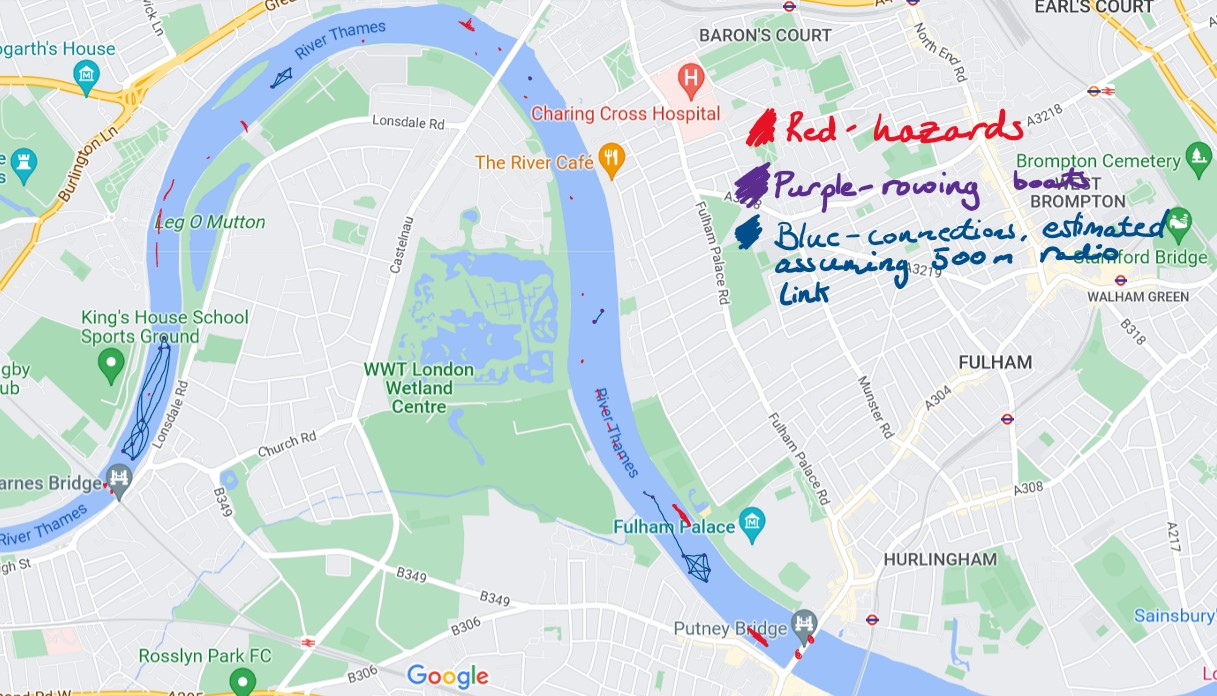
\includegraphics[scale=0.4]{mapsmarked.jpg}
\end{center}
\end{figure}
\begin{figure}[h]
\begin{center}
\caption{The network of rowing boats in an abstracted form}
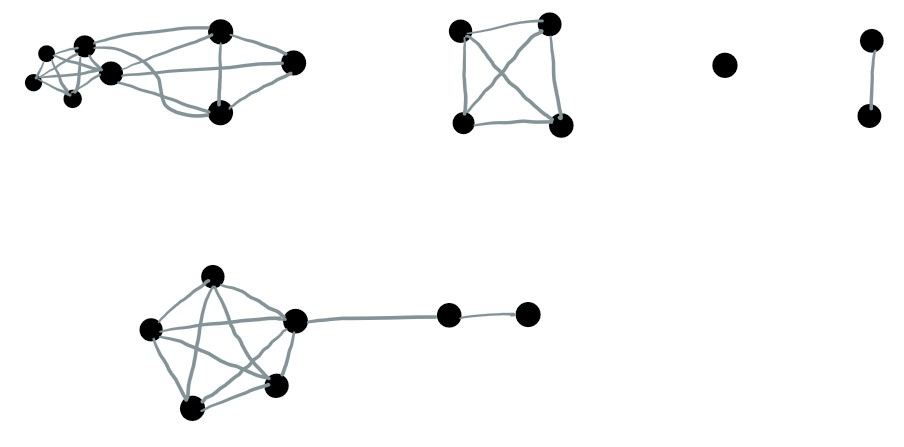
\includegraphics[scale=0.5]{lines.jpg}
\end{center}
\end{figure}
\FloatBarrier The final three requirements I identified as my success criteria were:
\begin{enumerate}
\item The Epidemic routing protocol is implemented on the network 
\item An application layer to demonstrate the utility of the network has been implemented
\item An evaluation of the performance of the network has been carried out
\end{enumerate}
All of these requirements have been implemented during this project. The finer details of this are in the Implementation chapter. \\ \\ I laid out several extension tasks. Some of them were drawn from my research into networking protocols other than Epidemic. For instance, I wanted to use a metric for transmission quality -- received strength signal indicator (RSSI) in radio communication -- to influence whether an anti-entropy session was initiated. Additionally, the GPS location could be used, either by only contacting nearby nodes to increase the probability that an anti-entropy session is successful, or prioritising sending messages about new obstacles to nodes that are near these obstacles. While time constraints have not allowed me to implement these extensions, I have implemented an extension allowing messages to have two priorities -- normal and urgent. This is also detailed in the Implementation chapter. 

\section{System Design}
Having decided on the Epidemic routing protocol, I planned the structure of the software that would run on each node. I knew that the Raspberry Pi Pico uses the RP2040 chip, containing two cores. To make best use of the hardware, I decided to design application and networking threads that would run on each core, with global data structures and concurrency control to pass messages between the two layers and allow both of them to access the GPS board. \\ \\
TODO you should talk about the flooding state machine you designed and the similarities between eidemic and flooding \\ \\ 
The application thread is responsible for notifying the user when they are too close to an obstacle. It also takes input from the user, generating new obstacles when a button is pressed. The initial state machine is shown in Figure 2.4. The a time to live (TTL) for each obstacle. If the object is permanent, such as a bridge, the TTL is set to $-1$, indicating that it should never be removed.
\begin{figure}[h]
\begin{center}
\caption{The initial state machine for the application thread}
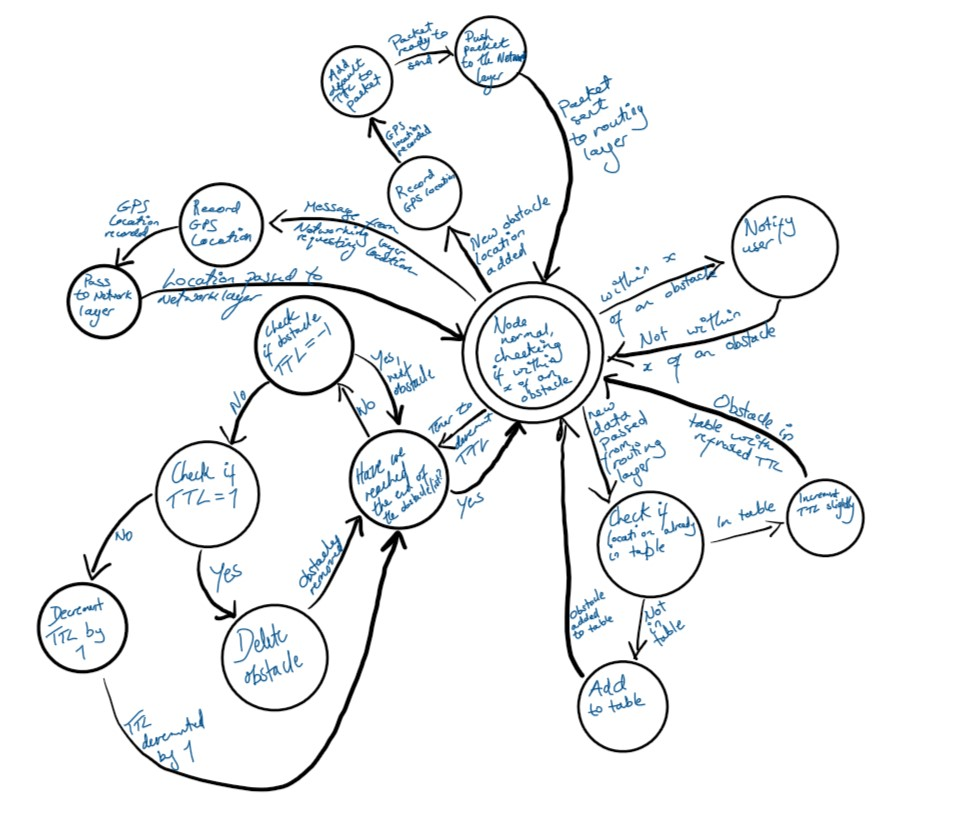
\includegraphics[scale=0.5]{appThread.jpg}
\end{center}
\end{figure}
\FloatBarrier
The networking thread contains the implementation of Epidemic with media access control. While routing and medium access control are typically handled separately -- in the OSI model they are in the second and third layers respectively -- they were considered together for my project to prevent work being repeated and use the limited computing resources available most effectively. This means that the implementation of Epidemic will also change. Not only will the node refuse to send any messages after hearing a CTS for a set period of time, or until it hears an ACK, I also integrated the message vector exchange at the start of an anti-entropy session into the CTS and RTS messages. This minimised the number of packets sent over the network, reducing the overall probability of collisions or errors in transmission. This state machine has changed slightly since it was first designed, with the changes and the decisions behind them being documented in the Implementation chapter. 
\begin{figure}[h]
\begin{center}
\caption{The initial state machine for the networking thread}
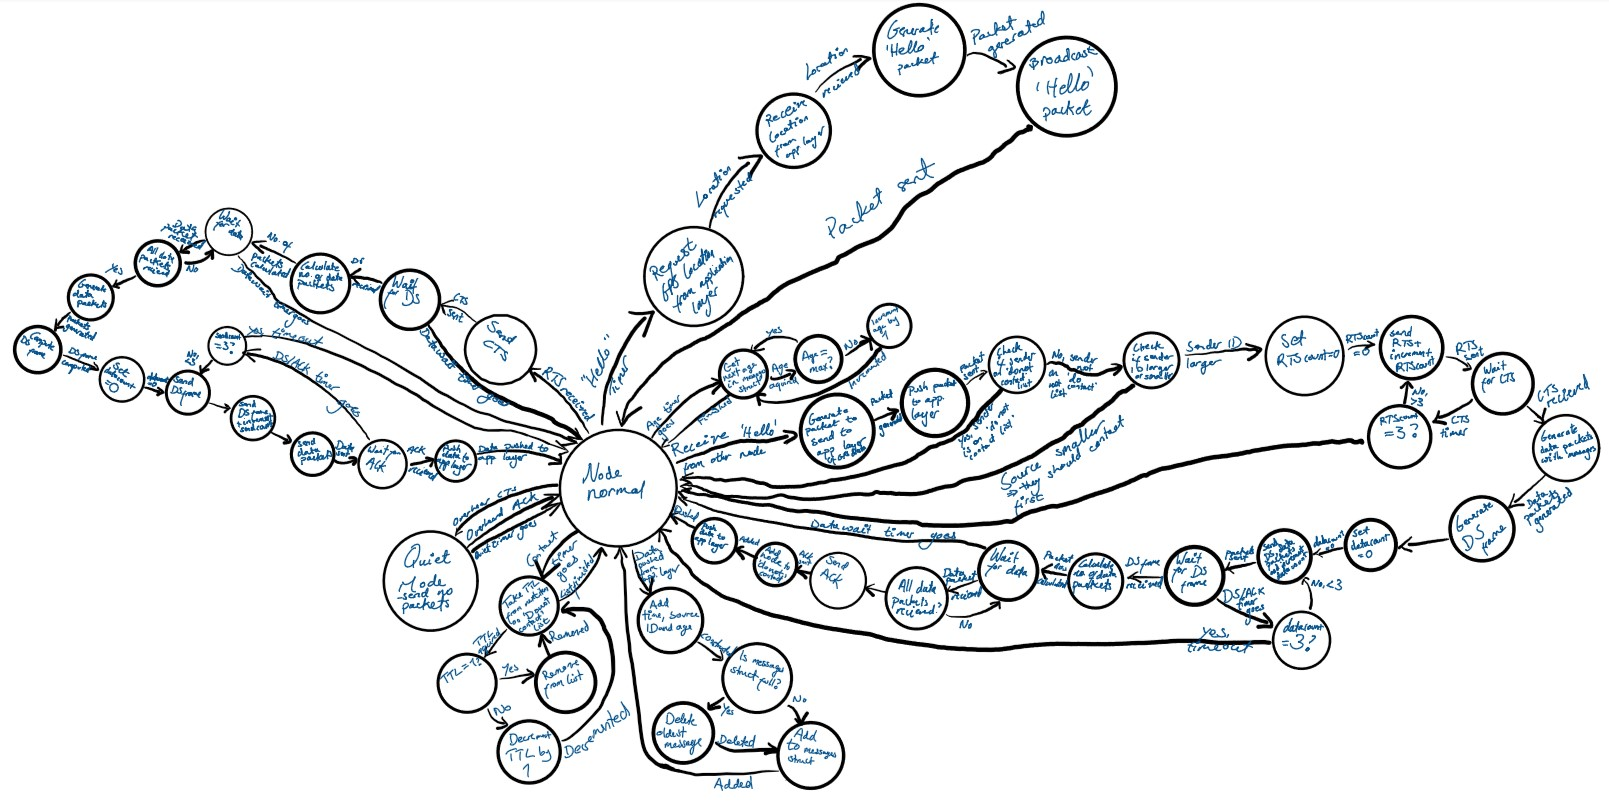
\includegraphics[scale=0.5]{net.jpg}
\end{center}
\end{figure}
\FloatBarrier
TODO -- talk about data structures -- The data structures designed to communicate messages between one thread and the other are  \\ \\
While these state machines were broadly implemented, the overall structure of the software changed, with only one thread running due to the limitations of CircuitPython and difficulties transitioning into MicroPython. This decision and the reasoning behind it is detailed in the Implementation chapter. 

%%% IMPLEMENTATION %%%
\newchapter{3}{Implementation}


%%% EVALUATION %%%
\newchapter{4}{Evaluation}
Evaluation was done (mostly) according to the plan in appendix. It was split into evaluation of the MANET and the whole system.

\section{Evaluating the MANET}
Break this down into smaller sections -- heavily quanitfy your results

\section{Evaluating the System}
We can def call this something better than the system? Idk the whole project, a more holistic evaluation? Emphasise that while the use case is kinda huge and untestable you tested within these restrictions and these parameters were met

%%% CONCLUSION %%%
\newchapter{5}{Conclusion}
What did this project do? The project met and exceeded the success criteria.

\section{Achievements}
What have you done?
In this project I have 

The evaluation shows that. This project is weak in. 

\section{Learning}
Aka lessons learnt / what I would do differently last time
Probably spent too much time researching BATMAN when it didn't really fit the parameters
Hardware is hard Just a stupid amount about radios and microprocessors

\section{Future Work}
I laid out several extension tasks. Some of them were drawn from my research into networking protocols other than Epidemic. For instance, I wanted to use a metric for transmission quality -- received strength signal indicator (RSSI) in radio communication -- to influence whether an anti-entropy session was initiated. Additionally, the GPS location could be used, either by only contacting nearby nodes to increase the probability that an anti-entropy session is successful, or prioritising sending messages about new obstacles to nodes that are near these obstacles. 
Encryption 
The success of my project will be defined by completion of the core criteria listed above. If there is
time, I have set further challenges:
1. Case studies on the path and timing of individual packets are performed
2. The network is further evaluated by examining the power consumption of individual nodes as
a proxy metric for traffic passing through a node
3. The User Interface of the device is evaluated
4. The application layer is further enhanced, using heuristics and extra data such as angle of
attack from GPS and combining sensor data
5. The routing layer is further enhanced by passing additional data, such as location awareness,
to the routing protocol
Okay so we never shut anything down in a safe ish way -- just kinda pull the plug and fuck off... ? Actually you should definately implement an editing of the Config file so we DO BETTER


%%% BIBLIOGRAPHY  %%%
\addcontentsline{toc}{chapter}{Bibliography}
%\bibliography{refs}


%%% APPENDICES %%%
\chapter*{Appendices}
\addcontentsline{toc}{chapter}{Appendices}  

\section*{A -- Guide to Building a Node}
\label{appendixA}
\addcontentsline{toc}{section}{A -- Guide to Building a Node}  
\setcounter{chapter}{0}
\setcounter{figure}{0}

\newpage
\section*{B -- Evaluation}
\label{appendixB}
\addcontentsline{toc}{section}{B -- Evaluation}  
\setcounter{figure}{0}
\input{evaluationPlan}

\newpage
\section*{C -- Progress Report}
\label{appendixC}
\addcontentsline{toc}{section}{C -- Progress Report}  
\setcounter{figure}{0}
\input{progressReport}

\newpage
\section*{D -- Project Proposal}
\label{appendixD}
\addcontentsline{toc}{section}{D -- Project Proposal}  
\setcounter{figure}{0}
\input{phase3}

\end{document}
%\frenchspacing			to get rid of the double spaces after full stops
%\graphicspath{}			if you have trouble getting images in the thing, asks for graphics in the same folder
\usepackage{caption}
\captionsetup{justification=raggedright,singlelinecheck=false}
 \usepackage[none]{hyphenat}

\begin{document}
\begin{center}
\Huge{Part II Project - Progress Report} \\
\Large{\today} \\
\end{center}
\textbf{Name:} Alex Riddell-Webster \\
\textbf{College:} Murray Edwards \\
\textbf{Email Address:} ahr38@cam.ac.uk \\
\textbf{Director of Studies:} Luana Bulat \\
\textbf{Supervisor:} Matthew Ireland \\
\textbf{UTO:} Professor Jon Crowcroft\\
\textbf{Overseers:}  Ferenc Huszar and Andreas Vlachos \\
\textbf{Title:} A MANET to Facilitate Collision Avoidance in Rowing Boats
\vspace{20px}\\
My project, a mobile ad-hoc network (MANET) to facilitate collision avoidance in rowing boats, attempts to reduce the frequency of rowing boat collisions. The technical core of the project is the Epidemic routing protocol \cite{epidemic}, modified to include medium access control based on the Multiple Access with Collision Avoidance for Wireless (MACAW) protocol \cite{macaw}. Both medium access control and Epidemic are implemented in the by the same state machine, to simplify the implementation and prevent work being repeated -- a waste of the limited resources on the Raspberry Pi Pico \cite{pico}. The initial state machine is shown in Figure 1, although it has been changed during implementation. Most notably, data send (DS) packets have been removed and the information being put into the data packets to reduce the number of packets sent. \\

\begin{figure}[h]
\caption{Network state machine}
\begin{center}
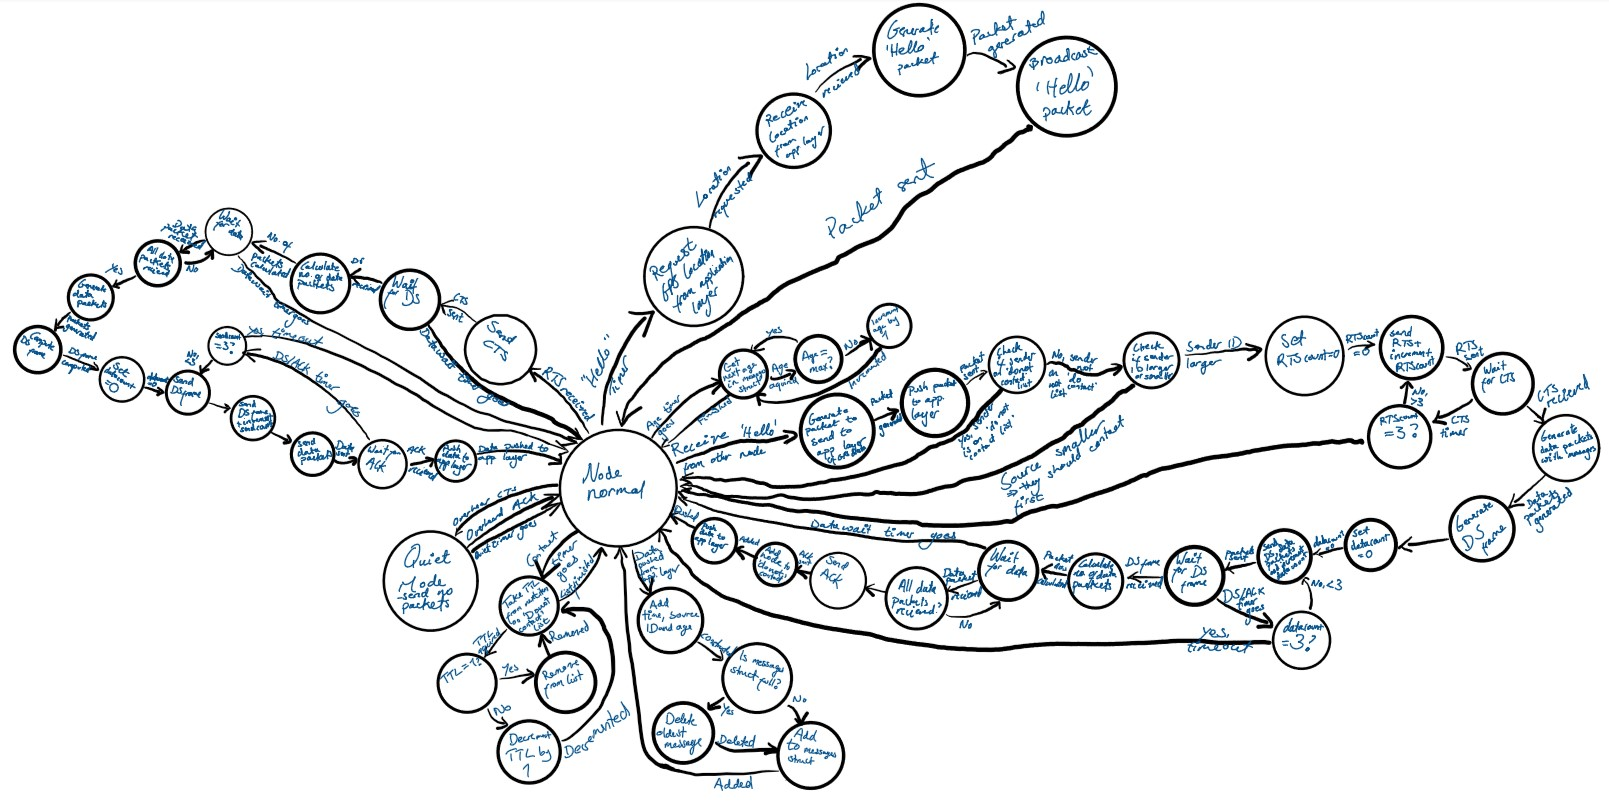
\includegraphics[scale=0.4]{net.jpg}
\end{center}
\end{figure}

Construction of the MANET is going well. It has been constructed in hardware, working with the Raspberry Pi Pico, an ARM-based microcontroller without an operating system \cite{pico} and RFM69 radio. I have finished the networking machine so am currently tweaking and evaluating the network state machine while finishing the application machine. As the network has a physical implementation, I intend to test the network on rowing boats, the environment it would be used. 

To ensure the network was delay tolerant, I ran a test with three nodes, $A$, $B$ and $C$. At the start, nodes $A$ and $B$ were in range of each other and node $C$ was out of range. I set node $A$ up to generate random messages every 40 seconds, with a time to live (TTL) greater than 2 so the messages would survive for two `hops' across the network. I then moved node $B$ out of range of node $A$ and into range of node $C$, which then displayed any messages it received so I could check that they were the same as those generated by $A$, with a reduced TTL. Figure 2 shows the setup.
\begin{figure}[h]
\caption{Using three nodes to check the network is delay tolerant}
\begin{center}
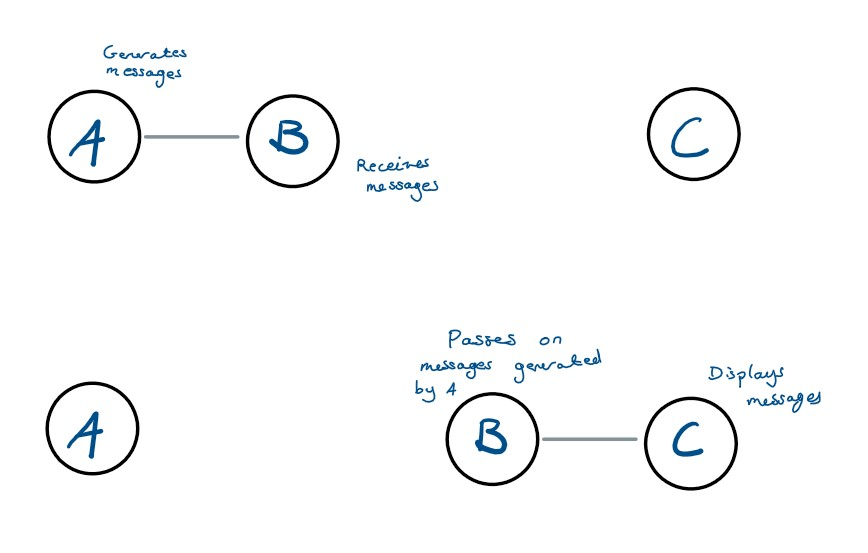
\includegraphics[scale=0.4]{test1.jpg}
\end{center}
\end{figure} \\
Another test involved four connected nodes, $A$, $B$, $C$, and $D$, where the transmit power of each node was significantly reduced, so each node had at most two connections. Node $A$ generated messages, and I checked to see if $D$ received them. I will use a similar set up in the future to test the percentage delivery and latency of packets. The setup is shown in Figure 3.
\begin{figure}[h]
\caption{Using four nodes to check the network can transfer packets over several links}
\begin{center}
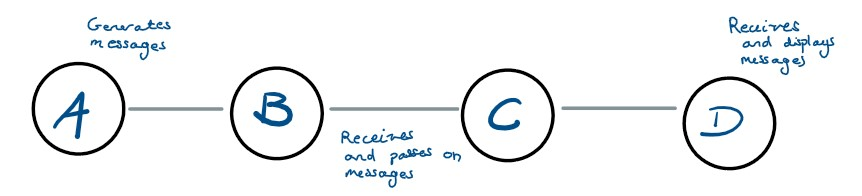
\includegraphics[scale=0.4]{test2.jpg}
\end{center}
\end{figure} \\

The most significant obstacles have been in radio communication. The FIFO buffer on the RFM69 was occasionally being overwritten as the controlling library was not clearing the FIFO. I modified the library to clear the buffer and allow the sending of fixed length packets. Changing to fixed length packets (64 bytes, the maximum length of the FIFO) allowed for more reliable communication. Additionally, CircuitPython (the language in which AdaFruit's libraries are written) does not support interrupts. To work around this, I poll to see if a condition is met when a corresponding timer elapses. \\

Given the work completed so far, I am two weeks behind the timetable laid out in October. As I am working on the application machine and evaluation of the network in parallel, the project will likely be back on timetable by mid-February.

The remaining work is first to finish the application machine and evaluate the MANET. Evaluation metrics will include the percentage of received packets, transfer delay and variance, and the time taken to propagate messages in a previously segmented network. Finally, I will pull the application and network machines together, running them on the two cores in the Pico, with concurrency control over key data structures and the GPS chip. A concern here is the Adafruit Blinka libraries allowing interoperability between CircuitPython and MicroPython \cite{blinka}, given the errors and incompleteness found in other libraries. 

\begin{thebibliography}{9}
\bibitem{epidemic} Epidemic Routing for Partially-Connected Ad Hoc Networks. Vahdat, A, Becker, D. Duke University. 2000.
\bibitem{macaw} MACAW: A Media Access Protocol for Wireless LAN's. Bharghavan, V, Demers, A, Shenker, S, Zhang, L. ACM SIGCOMM Conference. 1994.
\bibitem{pico} RP2040 Datasheet A microcontroller by Raspberry Pi. Raspberry Pi Ltd. 2022.
\bibitem{blinka} GitHub - adafuit/Adafruit\_Blinka: Add CircuitPython hardware API and libraries to MicroPython \& CPython devices. \url{https://github.com/adafruit/Adafruit_Blinka}. Adafruit Industries. GitHub. Accessed January 2023. 
\end{thebibliography}

\end{document}








\newpage
\section*{D -- Project Proposal}
\label{appendixD}
\addcontentsline{toc}{section}{D -- Project Proposal}  
\setcounter{figure}{0}
\input{phase3}

\end{document}
%\frenchspacing			to get rid of the double spaces after full stops
%\graphicspath{}			if you have trouble getting images in the thing, asks for graphics in the same folder
\usepackage{caption}
\usepackage{placeins}
\captionsetup{justification=raggedright,singlelinecheck=false}
\usepackage[none]{hyphenat}

\begin{document}
\begin{center}
\Huge{Part II Project - Plan for Evaluation} \par
\Large{\today} \par
\end{center}
\par
\par

\section{Overview}
The evaluation for the mobile ad-hoc network (MANET) will be split into two parts -- first the evaluation for the pure MANET and a whole system evaluation. The evaluation of the MANET will examine the implementation of Epidemic, the delay tolerant networking protocol will be checked for correctness and performance. The system evaluation will look at the MANET in the context of the use case, on the water.  \\

All data will be logged on the node in a CSV file with columns \\ \verb'Node Address, Time, Time Since Node Startup, Event Type, Event Information' \\ where the Event Information varies with the event being logged and may contain the GPS location and message keys. This data will then be analysed on my device using Python code.

\section{Evaluating the MANET}
These tests be conducted in a field, as this will give an outdoor environment similar to the use case, but I will be able to better control the conditions the node is in. They will use four nodes, as this is the maximum number of nodes we can accurately calculate time for. Two nodes will use GPS to find the current time and two will use the serial connection to laptops to calculate the time. These tests will be conducted first on a small scale, with short tests using a small number of nodes, to ensure the tests can be run. After this has been confirmed, the tests will be run for a longer time with the maximum number of nodes. 

The tests can then be compared to the evaluation in the initial epidemic paper \cite{epidemic}, which simulated the nodes with 50 mobile nodes in a 1500 x 300 m space using the Monarch extensions to the ns-2 packet-level simulator rather than hardware as I am doing. Evaluation metrics examined included message delivery latency, delivery rate, the average and maximum number of hops a message took to get to a node.

The first test will be the percentage of packets delivered in the four node network. This will be time limited (i.e. if a message is not received in x minutes, it is considered undelivered). Nodes will randomly generate a new message every second, for a total of 25 messages, mirroring the structure of testing used in Vahdat and Becker's paper \cite{epidemic}. The nodes will be in a box of area $20m^2$ with the range of the radios reduced to approximately $5m$ to simulate the environment in which the system will be used. The nodes will move constantly.

Next, the transfer delay will be measured. This will be the average time taken for each message to be delivered, and will use the same setup as percentage of packets delivered testing.

\begin{figure}[h]
\caption{The setup and axes for delivery rate and transfer delay}
\begin{center}
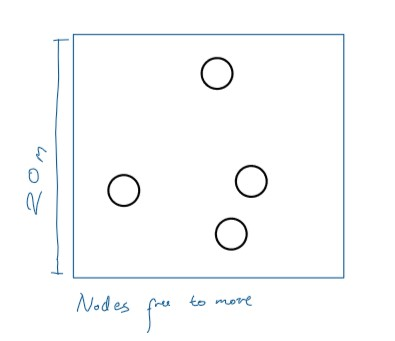
\includegraphics[scale=0.5]{transfer.jpg}
\end{center}
\end{figure}


Finally, the time taken to propagate messages after partition will be measured. This will include one-sided, asymmetric partitions, where only one set of nodes has messages the other set has not seen. It will also include symmetric partitions, where both sets of nodes have messages the other set has not seen. The number of unseen messages will be increased and each test will be run five times.

\begin{figure}[h]
\caption{The setup and axes for partition testing}
\begin{center}
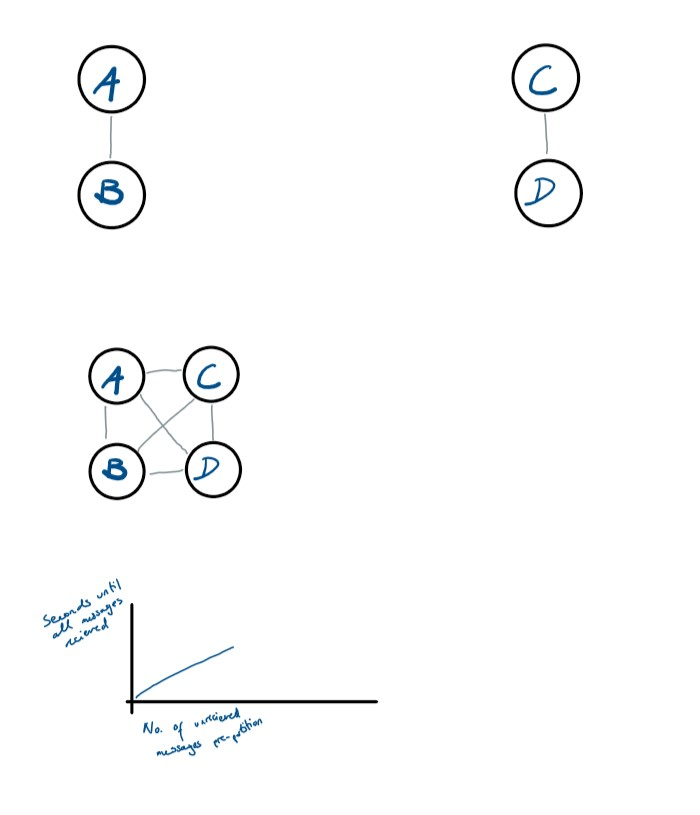
\includegraphics[scale=0.3]{partition.jpg}
\end{center}
\end{figure}


%sketch out graphs you will use
%Add pictures of the node teting setup 
%What will be evaluated and how?
%How to evaluate correctness? 
%How to do sensitivity on the data / metrics - how certain are we that this works..? 

\FloatBarrier
\section{Evaluating the System}
This will be performed on the water, the environment the MANET will be used in, after a `dry run' on land to ensure there are no obvious flaws with the system. 
To examine the use of the system and how long it takes messages to arrive at other nodes, a well known obstacle has been selected. This is the red buoy at 51.48236626931181, -0.22641424521527762, shown below \cite{maps}. Using the time given from the GPS chips, we can then map the locations and time since the obstacle was added that other nodes receive messages about the buoy. This experiment will be run multiple times to gather a sufficient volume of data about the propagation of new obstacles. \\

Additionally, this will allow me to look at the behaviour of users when adding a new obstacle then tweak the MANET to fit. While there is a ground truth about the location of an obstacle, it is likely that most users will not be directly above the obstacle when they log it. 

\begin{figure}[h]
\caption{The location of the `red buoy' obstacle \cite{maps}}
\begin{center}
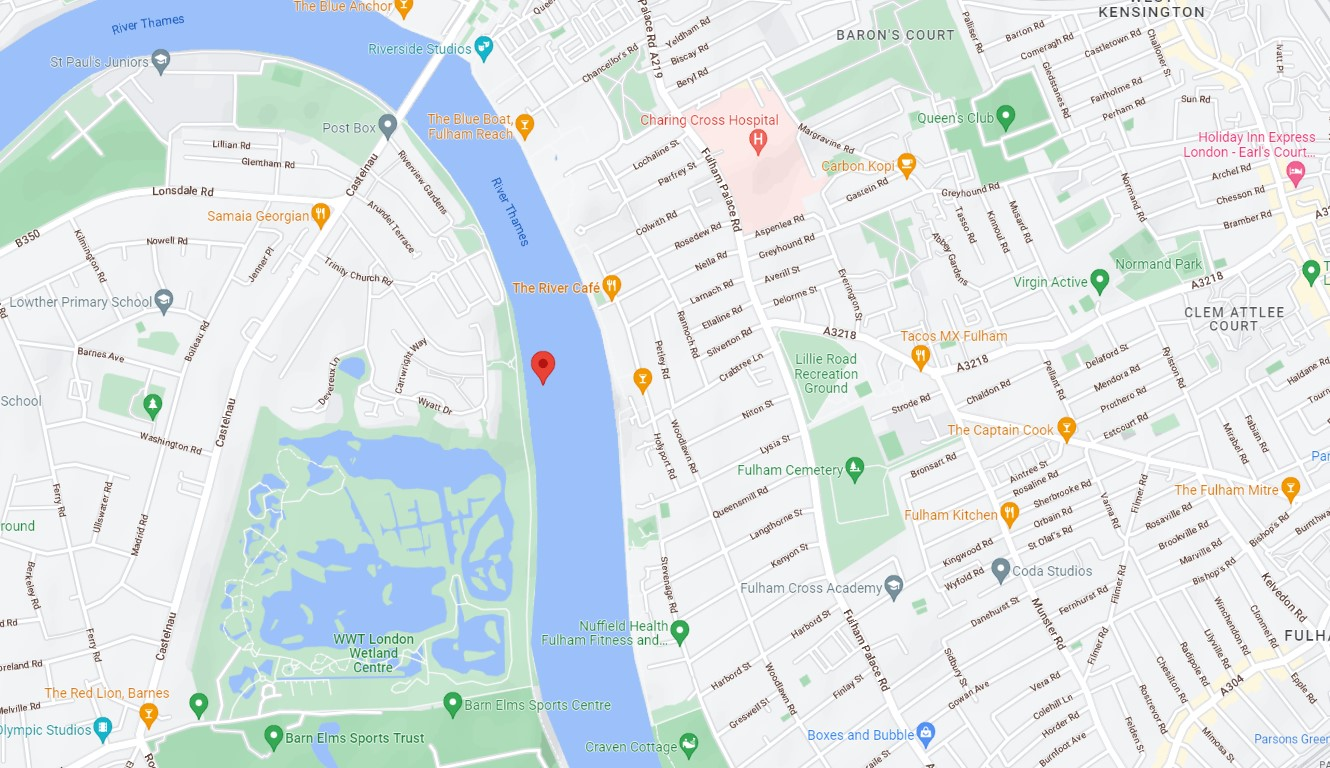
\includegraphics[scale=0.3]{buoy.jpg}
\end{center}
\end{figure}

\begin{figure}[h]
\caption{An image of the `red buoy' obstacle \cite{myphoto}}
\begin{center}
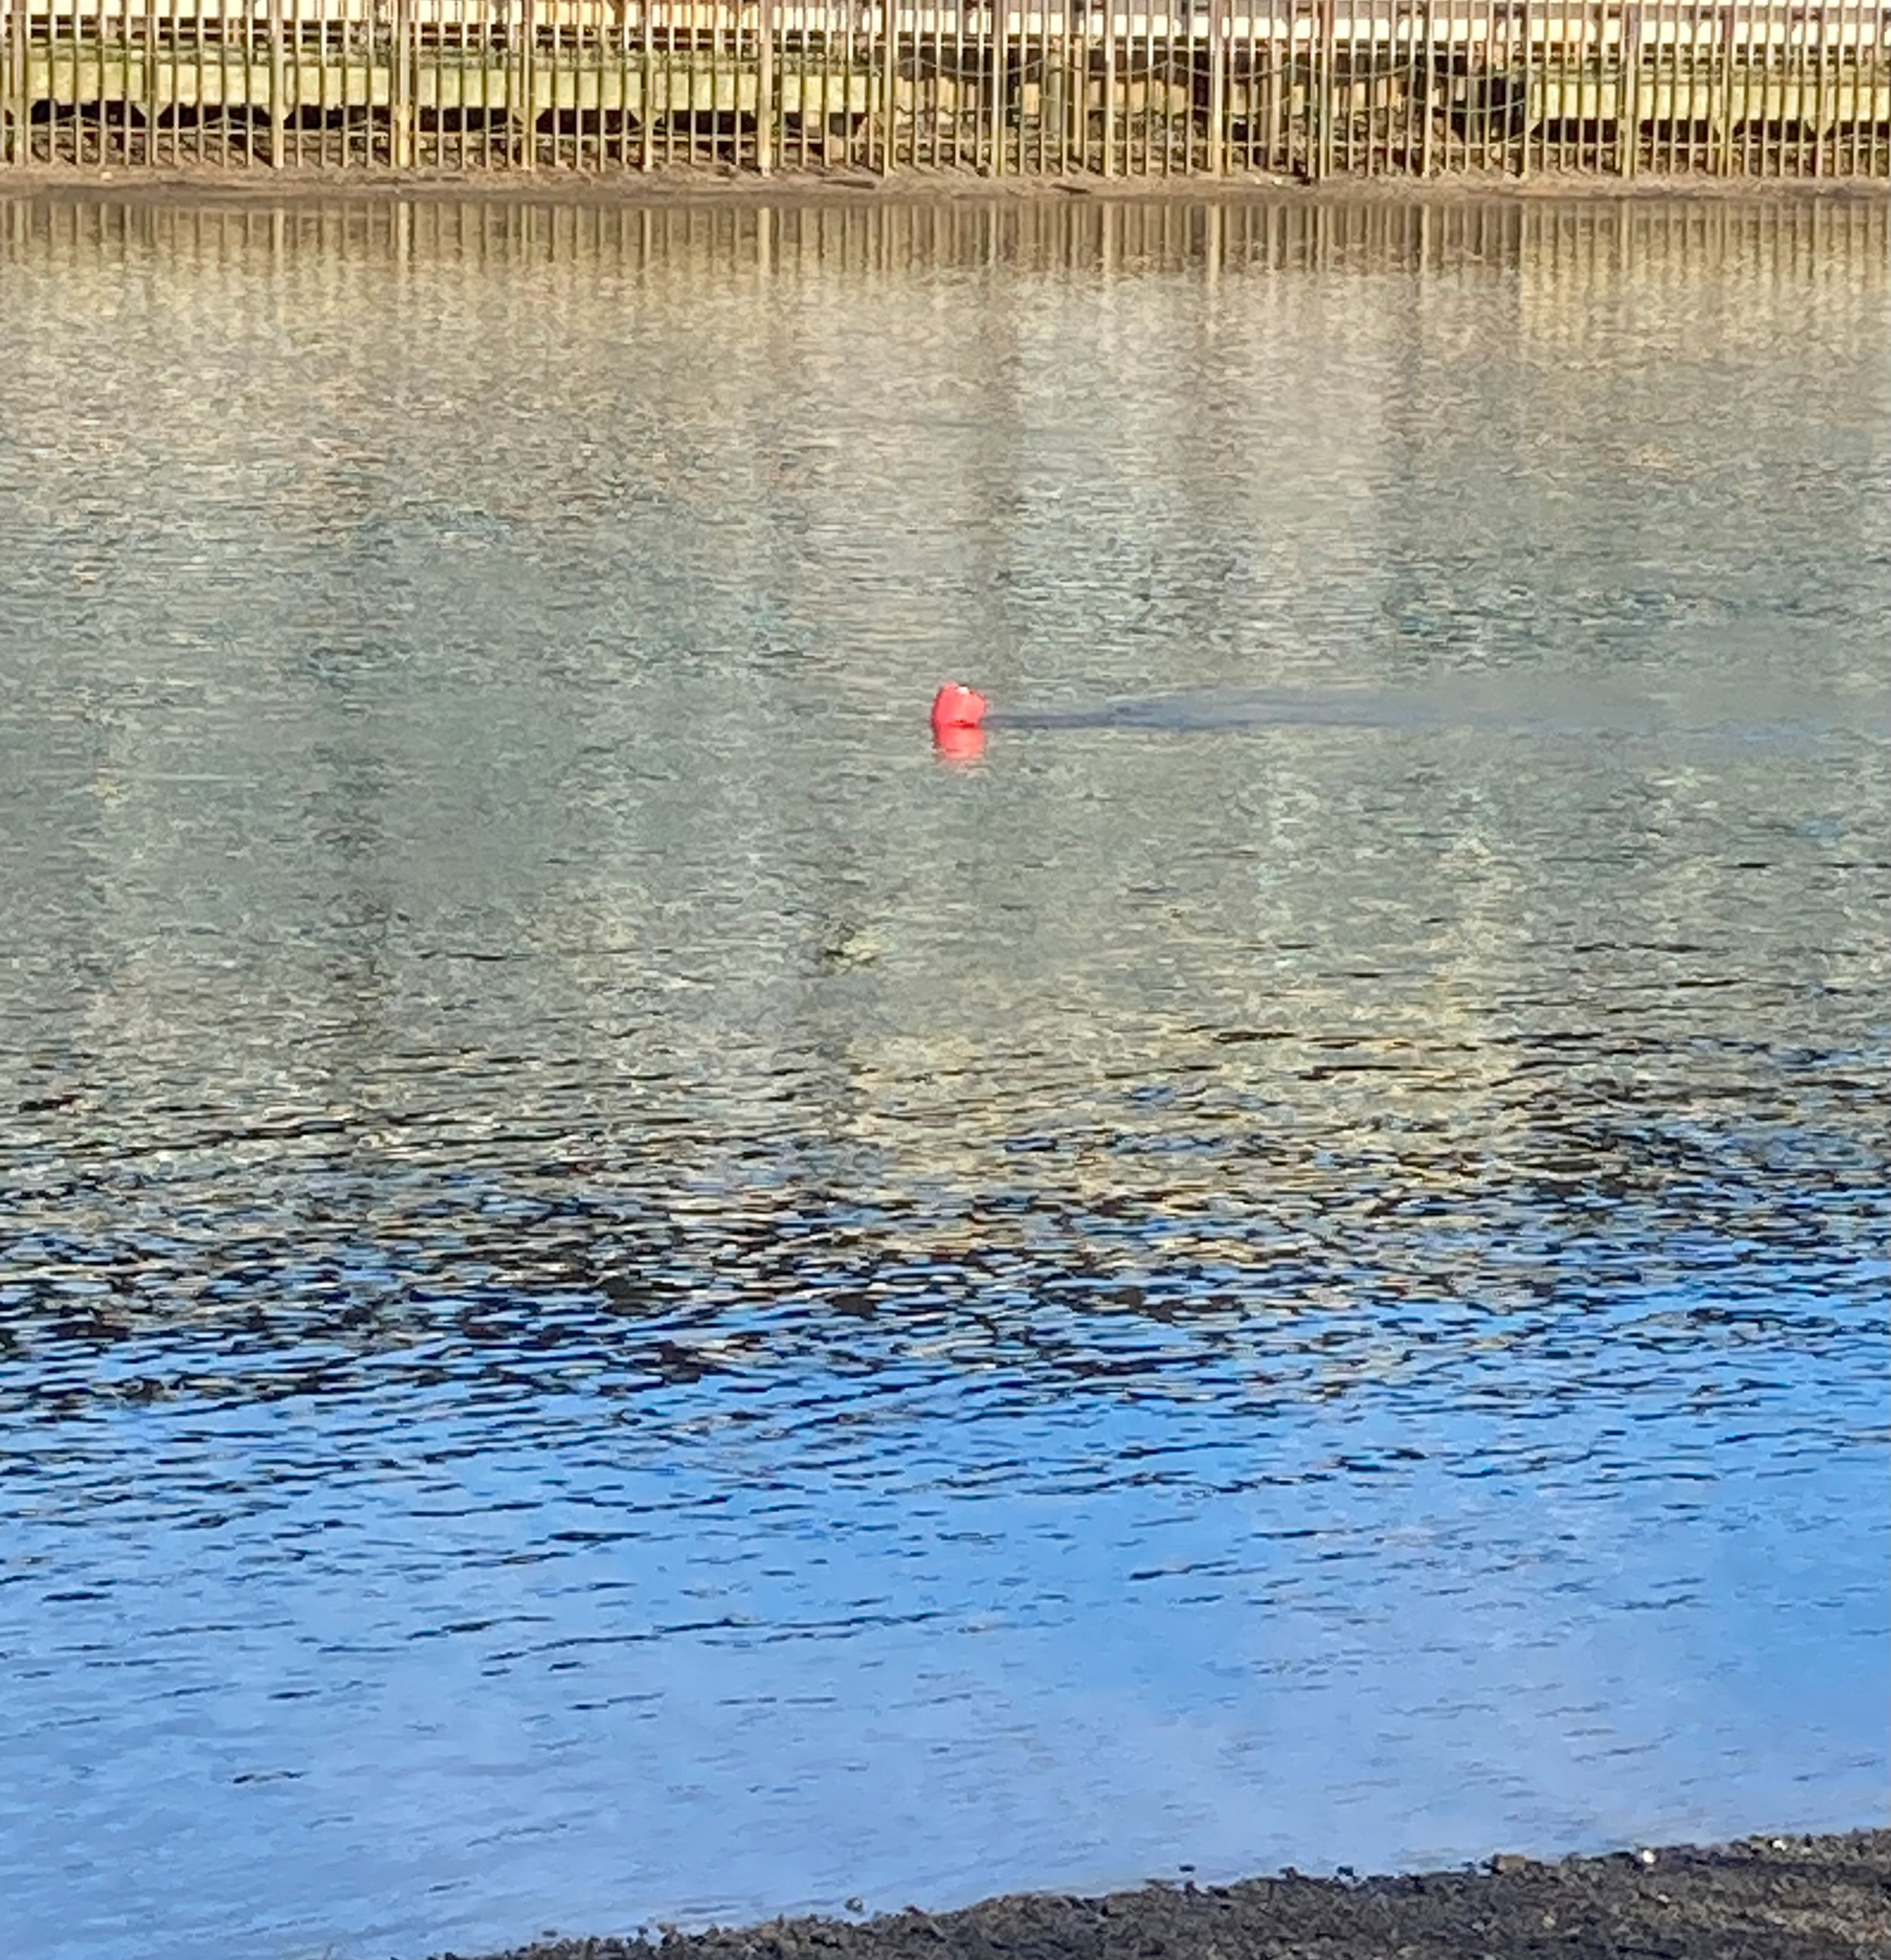
\includegraphics[scale=0.1]{buoy2.jpg}
\end{center}
\end{figure}
\FloatBarrier


\section{Extensions}
If there is sufficient time, further evaluation can be performed on the MANET. This will be structured in a similar way to the tests in the `Evaluating the MANET'. Bandwidth will be tested in a fully connected network, where the number of messages per second transferred between two nodes may be found by generating random packets at set intervals at one node (node A shown below), and seeing how many are passed to another node (node B below). 
This test could then be performed with both nodes generating and receiving messages, to examine bandwidth on a two way connection.\\
\begin{figure}[h]
\caption{The setup and expected graph for testing bandwidth}
\begin{center}
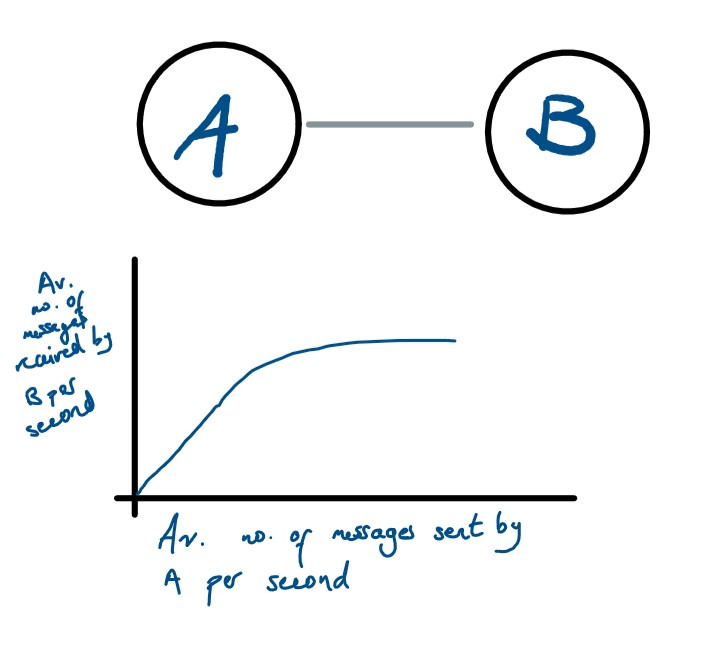
\includegraphics[scale=0.3]{bandwidth.jpg}
\end{center}
\end{figure}

Further extensions to the system evaluation will include a questionnaire for those who use the device, covering a range of users, including both coxes in coxed boats and rowers in coxless boats. 

\FloatBarrier
\vspace{10px}
\begin{thebibliography}{9} 
\bibitem{maps}Google Maps. 51.4823, -0.2264. [Online] Available at: \url{https://www.google.co.uk/maps/place/51%C2%B028'56.5%22N+0%C2%B013'35.1%22W/@51.4820341,-0.2295313,15.5z/data=!4m4!3m3!8m2!3d51.4823663!4d-0.2264142!5m1!1e4} [Accessed March 2023]

\bibitem{myphoto}Riddell-Webster, A. Red buoy. Taken March 2023. 

\bibitem{epidemic} Vahdat, A, Becker, D. Epidemic Routing for Partially-Connected Ad Hoc Networks. Published 2000. Duke University.
\end{thebibliography}

\end{document}






